% Created 2019-07-02 Tue 02:49
% Intended LaTeX compiler: pdflatex
\documentclass[11pt]{article}
\usepackage[utf8]{inputenc}
\usepackage[T1]{fontenc}
\usepackage{graphicx}
\usepackage{grffile}
\usepackage{longtable}
\usepackage{wrapfig}
\usepackage{rotating}
\usepackage[normalem]{ulem}
\usepackage{amsmath}
\usepackage{textcomp}
\usepackage{amssymb}
\usepackage{capt-of}
\usepackage{hyperref}
\author{Heitor Lourenço Werneck \\{\href{mailto:heitorwerneck@hotmail.com}{heitorwerneck@hotmail.com}}}
\usepackage[portuguese]{babel}
\usepackage{mathtools}
\usepackage[binary-units=true]{siunitx}
\usepackage[top=0.5cm,bottom=1.5cm,left=2cm,right=2cm]{geometry}
\usepackage{mdframed}
\usepackage{listings}
\usepackage[noend]{algpseudocode}
\usepackage{algorithm}
\usepackage{tikz}
\usepackage{xcolor}
\usepackage{colortbl}
\usepackage{graphicx,wrapfig,lipsum}
\RequirePackage{fancyvrb}
\DefineVerbatimEnvironment{verbatim}{Verbatim}{fontsize=\small}
\usepackage[font=small,labelfont=bf]{caption} % Required for specifying captions to tables and figures
\usepackage[subrefformat=parens]{subcaption}
\date{1 de Julho de 2019}
\title{Algoritmos e Estrutura de Dados III (2019-1)\\\medskip
\large Trabalho Prático 4}
\hypersetup{
 pdfauthor={Heitor Lourenço Werneck},
 pdftitle={Algoritmos e Estrutura de Dados III (2019-1)},
 pdfkeywords={},
 pdfsubject={},
 pdfcreator={Emacs 26.2 (Org mode 9.1.9)}, 
 pdflang={Portuguese}}
\begin{document}

\maketitle
\usetikzlibrary{arrows, fit, matrix, positioning, shapes, backgrounds,intersections}
\usetikzlibrary{decorations.pathreplacing}
\usetikzlibrary{automata, positioning, arrows}
\usetikzlibrary{calc}
\newcommand{\ccb}{\cellcolor{blue}}
\newcommand{\ccc}{\cellcolor{gray}}
\newcommand{\ccr}{\cellcolor{red}}
\newcommand{\ccg}{\cellcolor{green}}
\newcommand{\ccbl}{\cellcolor{black}}
\newcommand{\cco}{\cellcolor{orange}}


\newcommand{\algruledefaultfactor}{.75}
\newcommand{\algstrut}[1][\algruledefaultfactor]{\vrule width 0pt
depth .25\baselineskip height #1\baselineskip\relax}
\newcommand*{\algrule}[1][\algorithmicindent]{\hspace*{.5em}\vrule\algstrut
\hspace*{\dimexpr#1-.5em}}
\DeclarePairedDelimiter\ceil{\lceil}{\rceil}
\DeclarePairedDelimiter\floor{\lfloor}{\rfloor}
\makeatletter
\newcount\ALG@printindent@tempcnta
\def\ALG@printindent{%
    \ifnum \theALG@nested>0% is there anything to print
    \ifx\ALG@text\ALG@x@notext% is this an end group without any text?
    % do nothing
    \else
    \unskip
    % draw a rule for each indent level
    \ALG@printindent@tempcnta=1
    \loop
    \algrule[\csname ALG@ind@\the\ALG@printindent@tempcnta\endcsname]%
    \advance \ALG@printindent@tempcnta 1
    \ifnum \ALG@printindent@tempcnta<\numexpr\theALG@nested+1\relax% can't do <=, so add one to RHS and use < instead
    \repeat
    \fi
    \fi
}%

\patchcmd{\ALG@doentity}{\noindent\hskip\ALG@tlm}{\ALG@printindent}{}{\errmessage{failed to patch}}

\AtBeginEnvironment{algorithmic}{\lineskip0pt}

\newcommand*\Let[2]{\State #1 $\gets$ #2}
\newcommand*\Stateh{\State \algstrut[1]}

\algnewcommand{\IfThenElse}[3]{% \IfThenElse{<if>}{<then>}{<else>}
  \State \algorithmicif\ #1\ \algorithmicthen\ #2\ \algorithmicelse\ #3}
\algnewcommand{\Break}[0]{\textbf{break}}
\makeatletter
\renewcommand{\ALG@name}{Algoritmo}
\renewcommand{\listalgorithmname}{Lista de\ALG@name s}
\makeatother
\lstset{
  basicstyle=\ttfamily,
  columns=fullflexible,
  frame=single,
  breaklines=true,
  postbreak=\mbox{\textcolor{red}{$\hookrightarrow$}\space},
}
\tikzstyle{block} = [rectangle, draw, 
    text width=5em, text centered]
\tikzstyle{elli} = [draw,ellipse,text width=5em,text centered]
\tikzstyle{decision} = [diamond, draw,text width=4.5em, text badly centered, node distance=3cm, inner sep=0pt]
\tikzstyle{line} = [draw, -latex',dashed]

\newcommand{\myDistance}{2.8cm}
\AtBeginEnvironment{algorithmic}{\footnotesize}
\section{Introdução}
\label{sec:orgaac6447}

O trabalho a ser apresentado consiste em desenvolver algoritmos de busca de padrão, exato e aproximado, avaliando o desempenho dos mesmos em diversos ambientes. A busca de padrão é formalizada do seguinte modo: Há um texto \(T[1..n]\) de largura \(n\) e o padrão é \(P[1..m]\) de largura \(m\leq n\). Também é assumido que os elementos de \(P\) e \(T\) tem como fonte de seus caracteres um dicionário \(\Sigma\) finito. O padrão \(P\) ocorre em \(T\) na posição \(x\) do texto se \(1\leq x \leq n-m+1\) e \(T[x..x+m-1]=P[1..m]\). Um texto vazio é denotado por \(\varepsilon\). \cite{cormen09_introd}

Busca de padrão é usada em busca por sequencias de DNA, análise de registro de sistemas de informação e também esta muito presente a utilização por usuários de computadores em buscas de texto na Internet.

Os algoritmos desenvolvidos para solução do problema foram: Boyer Moore Horspool (BMH); BMH Sunday (BMHS); Shift-And; Shift-And aproximado; BMHS paralelo.

\section{Estrutura de dados}
\label{sec:org74d5200}
Para o armazenamento do texto e padrão foi suposto que o texto de entrada será ASCII, logo foi criado o tipo \emph{CharType} que é o tipo primitivo \emph{unsigned char} da linguagem C que é usado para guardar tanto o texto quanto o padrão.
\begin{verbatim}
typedef unsigned char CharType;
\end{verbatim}

Também é importante notar que o tipo definido suporta somente um número constante de caracteres que varia de arquitetura para arquitetura. Como definido anteriormente, o dicionário possui um número finito de elementos.
Logo é definido o Tamanho do alfabeto como:

\begin{equation}
ALPHABETSIZE = |\Sigma| \coloneqq 256 = 2^{(sizeof(CharType)\cdot 8)}
\end{equation}

Outra estrutura criada que auxilia no ShiftAnd é o \emph{bitVector} que possui a seguinte definição: \cite{bitarrayclibrary}

\begin{verbatim}
typedef unsigned char WordType;
struct bitVector{
  size_t bits;
  WordType *vector;
};
\end{verbatim}

Sendo \texttt{size\_t bits} o número de bits utilizado pelo \texttt{WordType *vector} e \texttt{WordType *vector} a lista de bits por si.

Essa estrutura de dados é representada na figura \ref{fig:bitv}.

\begin{figure}
\begin{center}
\begin{tikzpicture}
\node (a) at (0,0){
  \begin{tabular}{ | l | c | c | c | c | c | c | r |}
    \hline
    MSB & & ...& & LSB\\ \hline
  \end{tabular}
};
\node[xshift=1.95cm] (b) at (a.east){
  \begin{tabular}{ | l | c | c | c | c | c | c | r |}
    \hline
    MSB & & ...& & LSB\\ \hline
  \end{tabular}
};
\node[xshift=0.20cm] (c) at (b.east){...};

\draw[decorate,decoration={brace, amplitude=10pt, raise=5pt, mirror}]
  (a.south west) to node[black,midway,below= 15pt] {$\beta =$ sizeof(WordType)$\cdot$ 8} (a.south east);

\draw[->,yshift=0.2cm,xshift=-2.3cm,line width=0.3mm,left of = a,xshift=1cm,yshift=0.27cm] (0,0) -- (9,0) node[anchor=south east] {Crescimento da lista de bits};

\draw[->,line width=0.3mm,left of = a,xshift=-3cm] (0,0) -- (1,0) node[anchor=south east] {Primeiro bit};

\end{tikzpicture}
\end{center}
\caption{Vetor de bits.(''MSB'': Bit mais significativo; ''LSB'': bit menos significativo.)}\label{fig:bitv}
\end{figure}

Todas operações binárias necessárias para o Shift-And foram implementadas. Ou seja: ou(|); e(\&); deslocamento para a direita(\(>>\)). Também outras funções foram implementadas para operar bit a bit: uma para definir como 1 o enésimo bit, outra para definir como 0 o enésimo bit e também mais uma para checar o enésimo bit.

\begin{verbatim}
bitVector* bVSetBit(bitVector* bitv,size_t bit);// Define como 1 enésimo bit
bitVector* bVClearBit(bitVector* bitv,size_t bit);// Define como 0 enésimo bit
bitVector* bVOr(bitVector* dest,bitVector* src1,bitVector* src2);// Operação logica ou
bitVector* bVAnd(bitVector* dest,bitVector* src1,bitVector* src2);// Operação logica e
bitVector* bVClearAll(bitVector* target);// Define como 0 todo o vetor de bits
bitVector* bVShiftLeft(bitVector* dest,bitVector* src,size_t shifts);// Deslocamento para esquerda
bitVector* bVShiftRight(bitVector* dest,bitVector* src,size_t shifts);// Deslocamento para a direita
int bVIsSetBit(bitVector* target,size_t bit);// Define como 1 enésimo bit
\end{verbatim}

\section{Solução}
\label{sec:orgc4be543}

\subsection{Boyer Moore Horspool}
\label{sec:org627a789}

Booyer Moore Horspool(BMH) é um algoritmo de casamento exato de padrão que compara um padrão da direita para a esquerda e passa pelo texto da esquerda para a direita. 

O preprocessamento necessário para o algoritmo é a criação de uma tabela que indica o deslocamento que poderá ser realizado. Quando comparado um caractere do texto ao do padrão, se for diferente ou haver um casamento irá haver um deslocamento de acordo com o caractere no texto correspondente ao ultimo caractere do padrão. A construção da tabela de deslocamento se da pelo modelo apresentado na equação \ref{eq:dbmh}.

\begin{equation}
d[x]=min\{ j \text{ tal que } j =m | (1 \leq j < m \& P[m-j]=x))
\label{eq:dbmh}
\end{equation}

O algoritmo \ref{alg:bmh} descreve o comportamento detalhadamente.

\begin{algorithm}
\textbf{Input:} $T[0..n-1], n, P[0..m-1], m, match[0..n-1]$
\textbf{Output:} $match[0..n-1]$
\caption{Boyer Moore Horspool.}\label{alg:bmh}
\begin{algorithmic}[1]
\Procedure{preProcessBMH}{$d,P,m$}
\For{$i=0$ to $ALPHABETSIZE-1$}
\State $d[i]\gets m$
\EndFor
\For{$i=0$ to $m-2$}
\State $d[P[i]]\gets m-i-1$
\EndFor
\EndProcedure
\Procedure{BMH}{$T,n,P,m,match$}
\State $match\gets \{0,...,0\}$
\State preProcessBMH($d,P,m$)
\State $i\gets m$
\While{$i\leq n$}
\State $base\gets i$
\State $j\gets m$
\While{$j>0 \land T[base-1] = P[j-1]$}
\State $j\gets j-1; base\gets base -1$
\EndWhile
\If{$j=0$}
\State $match[base]\gets true$
\EndIf
\State $i\gets i+d[T[i-1]]$
\EndWhile
\EndProcedure
\end{algorithmic}
\end{algorithm}

\subsection{Boyer Moore Horspool Sunday}
\label{sec:org51d6441}

O Boyer Moore Horspool Sunday(BMHS) é um algoritmo também de casamento exato de padrão. O algoritmo é bem similar ao BMH, porém apresenta algumas variantes. O BMHS usa uma abordagem diferente para o modelo de deslocamento. O endereçamento a tabela e dado pelo caractere no texto correspondente ao caractere após o último caractere do padrão. O modelo da tabela de deslocamento é a equação \ref{eq:dbmhs}.

\begin{equation}
d[x]=min\{ j \text{ tal que } j =m | (1 \leq j \leq m \& P[m+1-j]=x))
\label{eq:dbmhs}
\end{equation}

O algoritmo \ref{alg:bmhs} descreve o comportamento do BMHS detalhadamente.

\begin{algorithm}
\textbf{Input:} $T[0..n-1], n, P[0..m-1], m, match[0..n-1]$
\textbf{Output:} $match[0..n-1]$
\caption{Boyer Moore Horspool Sunday.}\label{alg:bmhs}
\begin{algorithmic}[1]
\Procedure{preProcessBMHS}{$d,P,m$}
\For{$i=0$ to $ALPHABETSIZE-1$}
\State $d[i]\gets m+1$
\EndFor
\For{$i=0$ to $m-1$}
\State $d[P[i]]\gets m-i$
\EndFor
\EndProcedure
\Procedure{BMHS}{$T,n,P,m,match$}
\State preProcessBMHS($d,P,m$)
\State $i\gets m$
\While{$i\leq n$}
\State $base\gets i$
\State $j\gets m$
\While{$j>0 \land T[base-1] = P[j-1]$}
\State $j\gets j-1; base\gets base -1$
\EndWhile
\If{$j=0$}
\State $match[base]\gets true$
\EndIf
\If{$i<n$}
\State $i\gets i+d[T[i]]$
\Else
\State \Break
\EndIf
\EndWhile
\EndProcedure
\end{algorithmic}
\end{algorithm}

\subsection{Shift-And}
\label{sec:orgf15063b}

O Shift-And é um algoritmo que explora operações que tiram proveito do tamanho da palavra da arquitetura utilizada, com isso consegue um paralelismo assim reduzindo o numero de operações que o algoritmo realiza em até um fator de \(\beta\). O Shift-And pode ser visto como uma simulação de um autômato não determinista que pesquisa pelo padrão no texto.

A modelagem do problema foi feita de um modo generalista, ou seja, para resolver o problema de casamento aproximado. O casamento exato é uma especificação desse problema e pode ser resolvido com um erro definido como zero. Ou seja, algoritmo exato: ShiftAnd\((T,n,P,m,0)\).(algoritmo \ref{alg:shiftand})

Um exemplo de autômato para casamento aproximado é mostrado na figura \ref{fig:automato1}. 

Um caractere quando é casado é representado pela aresta horizontal, a aresta vertical insere um caractere no padrão(\(R_{j-1}\)), a aresta diagonal continua substitui um caractere(\(R_{j-1}>>1\)) e a aresta diagonal tracejada remove(\(R^{'}_{j-1}>>1\)).

Cada linha j (\(0<j\leq error\)) do autômato representa um erro diferente, então o algoritmo ShiftAnd reúne essas linhas em uma palavra \(R_{j}\). Os vetores de bits \(R[0..error]\) são atualizados a cada caractere lido do texto e a simulação do autômato é feita através de operações em bits. 

Para simular esse autômato o Shift-And começa criando uma máscara de bits para cada palavra do alfabeto e quando um caractere é encontrado na enésima posição do texto é também definido como 1 na enésima posição da máscara de bits do carácter. É importante notar que as operações no vetor de bits dependem de como o vetor de bits é definido, a imagem \ref{fig:bitv} ilustra o modelo de vetor de bits utilizado nesse trabalho.

O seguinte modelo descreve o comportamento que deve ocorrer para realizar os casamentos a cada caractere na posição \(i\) do texto:(equação \ref{eq:shiftand})

\begin{equation}
\begin{aligned}
R^{'}_{0}=((R_{0}>>1)|1)\&mask[T[i]]\\
R^{'}_{j}=(R_{j}>>1)\&mask[T[i]]|R_{j-1}|(R_{j-1}>>1)|(R^{'}_{j-1}>>1)\\
\end{aligned}\label{eq:shiftand}
\end{equation}

Com a máscara definida é possível verificar os casamentos que vão ocorrendo no texto. O algoritmo \ref{alg:shiftand} descreve o comportamento detalhadamente.

\begin{algorithm}
\textbf{Input:} $T[0..n-1], n, P[0..m-1], m, match[0..n-1], error$
\textbf{Output:} $match[0..n-1]$
\caption{Shift-And.}\label{alg:shiftand}
\begin{algorithmic}[1]
\Procedure{ShiftAnd}{$T,n,P,m,match,error$}
\State $R1\gets 1$
\State $mask[0..ALPHABETSIZE-1]\gets \{0,...,0\},R[error+1]\gets \{0,...,0\}$
\For{$i=0$ to $m-1$}
\State $SetBit(mask[P[i]],i)$
\EndFor
\State $ClearAll(R[0]); aux \gets bitVectorNew(m)$
\For{$i=1$ to $error$}
\State $R[i]\gets R[i-1]$
\State $SetBit(R[i],i-1)$
\EndFor
\For{$i=0$ to $n-1$}
\State $Rprevious\gets R[0]$
\State $Rnew\gets$ $((Rprevious>>1)|R1)$ \&  $mask[T[i]]$
\State $R[0]\gets Rnew$
\For{$j=1$ to $error$}
\State $Rnew\gets ((R[j]>>1) \& mask[T[i]]) | Rprevious | Rprevious>>1 | Rnew>>1$
\State $Rprevious\gets R[j]$
\State $R[j]\gets Rnew|R1$
\EndFor
\If{$IsSetBit(Rnew,m-1) \land (n>i+1-m) \land (i+1-m \geq 0)$}
\State $match[i+1-m]\gets true$
\EndIf
\EndFor
\EndProcedure
\end{algorithmic}
\end{algorithm}

\begin{figure}
\begin{center}
\begin{tikzpicture}[auto,node distance=1.8cm,thick]
\node[state, initial,initial text=] (0) {0};
\node[state,right of=0] (1) {1};
\node[state,right of=1] (2) {2};
\node[state,right of=2] (3) {3};
\node[state,right of=3] (4) {4};
\node[state,right of=4,accepting] (5) {5};
\node[state,below of=0] (0') {0};
\node[state,right of=0'] (1') {1};
\node[state,right of=1'] (2') {2};
\node[state,right of=2'] (3') {3};
\node[state,right of=3'] (4') {4};
\node[state,right of=4',accepting] (5') {5};
\draw (0) edge[loop above,->] node{$\Sigma$} (0)
(0) edge[above,->] node{t} (1)
(1) edge[above,->] node{e} (2)
(2) edge[above,->] node{x} (3)
(3) edge[above,->] node{t} (4)
(4) edge[above,->] node{o} (5)
(0') edge[above,->] node{t} (1')
(1') edge[above,->] node{e} (2')
(2') edge[above,->] node{x} (3')
(3') edge[above,->] node{t} (4')
(4') edge[above,->] node{o} (5')
(0) edge[->] node{$\Sigma$} (0')
(1) edge[->] node{$\Sigma$} (1')
(2) edge[->] node{$\Sigma$} (2')
(3) edge[->] node{$\Sigma$} (3')
(4) edge[->] node{$\Sigma$} (4')
(5) edge[->] node{$\Sigma$} (5')
(0) edge[above,bend left=25,->,dashed] node{$\varepsilon$} (1')
(1) edge[above,bend left=25,->,dashed] node{$\varepsilon$} (2')
(2) edge[above,bend left=25,->,dashed] node{$\varepsilon$} (3')
(3) edge[above,bend left=25,->,dashed] node{$\varepsilon$} (4')
(4) edge[above,bend left=25,->,dashed] node{$\varepsilon$} (5')
(0) edge[above,bend right=5,->] node{$\Sigma$} (1')
(1) edge[above,bend right=5,->] node{$\Sigma$} (2')
(2) edge[above,bend right=5,->] node{$\Sigma$} (3')
(3) edge[above,bend right=5,->] node{$\Sigma$} (4')
(4) edge[above,bend right=5,->] node{$\Sigma$} (5');
\end{tikzpicture}
\end{center}
\caption{Autômato de busca com erro 1.}\label{fig:automato1}
\end{figure}

\subsection{BMHS Paralelo}
\label{sec:org39ceab6}
Algumas definições iniciais são necessárias para analisar o problema de paralelizar o BMHS. Seja \(p\) o número de processadores, \(P_i\) o processador \(i\), \(0\leq i < p\), \textbf{for all} .. \textbf{end for} ativa conjunto de processadores, \(n\) o tamanho do texto como já definido.

Para separar o problema do texto em partes é possível usar a seguinte formula para dividir o problema:
\begin{equation}
\alpha (i)=\text{Começo}(i) = \floor*{\frac{i\cdot n}{p}};\text{Fim}(i) = \floor*{\frac{(i+1)\cdot n}{p}}
\end{equation}

Esse tipo de divisão do texto não trata o caso que o padrão esta entre um bloco de texto e outro. Para tratar isso a formula do fim pode ser redefinida adicionando uma soma do tamanho do padrão menos um, deste modo será possível sempre obter o padrão. (equação \ref{eq:modelo2})

\begin{equation}
\omega (i)=\text{Fim}(i) = 
\begin{cases} 
\floor*{\frac{(i+1)\cdot n}{p}}-1+m &\text{se } i<p-1\\
\\
\floor*{\frac{(i+1)\cdot n}{p}} &\text{se } i=p-1
\end{cases}
\label{eq:modelo2}
\end{equation}

Essa formula define o começo e fim da busca para o BMHS. A posição real no texto T[0..n-1] é dada como: Começo \(= \alpha (i)\) e Fim  \(= \omega (i)-1\). A figura \ref{fig:exemploparalelo} exemplifica a divisão de blocos realizada.

\begin{figure}
\begin{center}
\begin{tikzpicture}[auto,node distance=0.7cm]
\node (a) at (0,0){
  \begin{tabular}{|l|c|c|c|c|c|c|c|c|c|c|c|c|c|c|c|r|}
    \hline
    o & i & o & l & a & h & e &l &l&o &y & o & h& o&l & a & '\textbackslash n ' \\ \hline
  \end{tabular}
};
\node (b)[below of= a] at (-3.6,0){
  \begin{tabular}{|l|c|c|c|c|r|}
    \hline
    o & i & \ccc o &\ccc l &\ccc a&h \\ \hline
  \end{tabular}
};

\node (c)[below of= b,xshift=2.35cm] {
  \begin{tabular}{|l|c|c|c|c|r|}
    \hline
    a & h & e & l & l & o  \\ \hline
  \end{tabular}
};

\node (d)[below of= c,xshift=2.48cm] {
  \begin{tabular}{|l|c|c|c|c|r|}
    \hline
    l & o & y & o & h & o  \\ \hline
  \end{tabular}
};

\node (e)[below of= d,xshift=2.37cm] {
  \begin{tabular}{|l|c|c|c|r|}
    \hline
    h &\ccc o & \ccc l & \ccc a & '\textbackslash n '  \\ \hline
  \end{tabular}
};
\end{tikzpicture}
\end{center}
\caption{Distribuição de dados pelos processadores com texto com n=17, p=4, P=ola.}\label{fig:exemploparalelo}
\end{figure}

Também é interessante caracterizar os blocos criados para paralelizar o algoritmo. O tamanho de cada bloco sem ser o ultimo é dado pela regra: \(\floor{n/numThreads+m-1}\)

logo o tamanho total de blocos é dado por: 
\begin{equation}
T(numThreads,n,m) = (numThreads-1)\cdot \floor*{\frac{n}{numThreads}+m-1}+n-\floor*{(numThreads-1)\cdot \frac{n}{numThreads}}
\end{equation}

Essa função de tamanho consegue mostrar o aumento de tamanho obtido por paralelizar o algoritmo. (\(T(numThreads,n,m)/n\))

Antes da criação do algoritmo definitivamente é necessário definir um limite superior de divisão de blocos. Esse limite é dado por \(\ceil{n/m}\) blocos pois a propriedade \(m\leq n\) deve se manter para não ocorrer de um bloco menor que \(m\) pois não há possibilidade de haver um casamento. Logo o número de threads máximo e necessário é \(\ceil{n/m}\). Com toda essa base o algoritmo \ref{alg:pbmh} é definido.

\begin{algorithm}
\textbf{Input:} $T[0..n-1], n, P[0..m-1], m, match[0..n-1]$
\textbf{Output:} $match[0..n-1]$
\caption{BMHS Paralelo.}\label{alg:pbmh}
\begin{algorithmic}[1]
\Procedure{PBMHS}{}
\State preProcessBMHS($d,P,m$)
\If{$numThreads>\ceil{n/m}$}
\State $numThreads = \ceil{n/m}$
\EndIf
\For{\textbf{all} $P_{i}$, $0 \leq i < numThreads$}
\State $begin\gets \alpha(i)$
\State $end\gets \omega(i)$
\State PBMHSF($T,n,P,m,match,d,begin,end$)
\EndFor
\EndProcedure

\Procedure{PBMHSF}{$T,n,P,m,match,d,begin,end$}
\State $i\gets begin+m$
\While{$i\leq end$}
\State $base\gets i$
\State $j\gets m$
\While{$j>0 \land T[base-1] = P[j-1]$}
\State $j\gets j-1; base\gets base -1$
\EndWhile
\If{$j=0$}
\State $match[base]\gets true$
\EndIf
\If{$i<n$}
\State $i\gets i+d[T[i]]$
\Else
\State \Break
\EndIf
\EndWhile
\EndProcedure
\end{algorithmic}
\end{algorithm}

\section{Análise de complexidade}
\label{sec:org75518ad}
\subsection{Complexidade de tempo}
\label{sec:orgb3e1ea0}
\subsubsection{BMH}
\label{sec:org1ada3f8}

\begin{equation}
\begin{aligned}
\text{preProcessBMH} \in O(|\Sigma|+m)\\
\text{BMH} \in O(n\cdot m+|\Sigma|+m)
\end{aligned}
\end{equation}
Simplificando a complexidade do algoritmo é dada por: \(O(n\cdot m)\). No melhor caso é \(O(n/m)\) e o caso esperado é \(O(n/m)\) \cite{galil79_improv_worst_case_runnin_time}, essas afirmações são compartilhadas pelo BMHS e BMHS Paralelo.

O pior caso desse algoritmo se expressa no exemplo dado na figura \ref{fig:exemplobmh}.

\begin{figure}
\centering
\begin{BVerbatim}
  T:aaaaaaaa
  P:aaaa
     aaaa
      aaaa
       aaaa
	aaaa
\end{BVerbatim}
\caption{Exemplo de execução BMH.}\label{fig:exemplobmh}
\end{figure}


\subsubsection{BMHS}
\label{sec:orga41f1c2}
\begin{equation}
\begin{aligned}
\text{preProcessBMHS} \in O(|\Sigma|+m)\\
\text{BMHS} \in O(n\cdot m+|\Sigma|+m)\\
\text{BMHS} \in O(n\cdot m)
\end{aligned}
\end{equation}

\subsubsection{Shift-And}
\label{sec:org3629f1e}
Para analisar a complexidade de tempo do ShiftAnd é necessário analisar a complexidade das operações binárias criadas para auxiliar. Seja \(bits\) o número de bits alocado para o vetor de bits, \(shifts\) é a quantidade de deslocamentos a serem realizados e \(\beta = sizeof(WordType)\cdot 8\) como definido na figura \ref{fig:bitv}.
\[
\begin{array}{cccccccc}
\hline bVSetBit & bVClearBit & bVOr & bVAnd & bVClearAll & bVShiftLeft & bVShiftRight & bVIsSetBit \\
\hline O(1) & O(1) & O(\frac{bits}{\beta}) & O(\frac{bits}{\beta}) & O(\frac{bits}{\beta}) & O(\frac{shifts\cdot bits}{\beta}) & O(\frac{shifts\cdot bits}{\beta}) & O(1) \\
\end{array}
\]

Para simplificar essa tabela somente com os termos necessários os termos constantes podem ser removidos, o termo \(\beta\) é uma constante logo pode ser removido, o shifts também tem um limite pois no máximo o deslocamento é do tamanho da palavra e nenhum comportamento diferente ocorre além disso logo a tabela pode ser reescrita como:

\begin{center}
\begin{tabular}{llllllll}
\hline
bVSetBit & bVClearBit & bVOr & bVAnd & bVClearAll & bVShiftLeft & bVShiftRight & bVIsSetBit\\
\hline
O(1) & O(1) & O(bits) & O(bits) & O(bits) & O(bits) & O(bits) & O(1)\\
\end{tabular}

\end{center}

O custo para inicializar as máscaras com 0 é \(O(|\Sigma|)\). O custo para inicializar os R's é \(O(error)\). No caso \(bits = m\) logo a complexidade do ShiftAnd será:

\begin{equation}
\begin{aligned}
O(m\cdot (|\Sigma|+error+ n\cdot (error+1)))\\
\text{ShiftAnd} \in O(m\cdot (|\Sigma|+ n\cdot (error+1)+error))\\
\text{ShiftAnd} \in O(m\cdot n\cdot error)
\end{aligned}
\end{equation}

Com um \(m\) menor que \(\beta\) ou pelo menos mantendo-se relativamente pequeno o algoritmo irá apresentar complexidade \(O(|\Sigma|+ n\cdot (error+1))\).

\subsubsection{BMHS Paralelo}
\label{sec:org9b13285}
A complexidade da criação das numThreads threads é \(O(numThreads)\) ou \(O(p)\). Sendo thread uma tarefa que um programa executa.

A complexidade é simplesmente \(PBMHS \in O(m\cdot n/p+p)\) pois o trabalho é distribuído para \(p\) processadores que conseguem trabalhar simultaneamente no problema.


\subsection{Complexidade de espaço}
\label{sec:org8bcb36c}

\subsubsection{BMH}
\label{sec:org230a8a9}
O algoritmo BMH somente aloca uma tabela de deslocamento com complexidade de espaço \(O(|\Sigma|)\). Logo sua complexidade é \(O(|\Sigma|)\).

\subsubsection{BMHS}
\label{sec:orgd5a2931}
O BMHS utiliza somente uma tabela de deslocamento assim como o BMH, sua complexidade de espaço é \(O(|\Sigma|)\).

\subsubsection{Shift-And}
\label{sec:org47dcd2a}
O ShiftAnd usa um vetor de máscara de bits que tem custo de espaço de \(O(m\cdot |\Sigma|)\) pois cada máscara para cada caractere deve ser do tamanho do padrão. Também é utilizado um vetor de vetor de bits para guardar os resultados do processo de casamento, esse vetor cresce de acordo com o número de erros permitidos no padrão logo sua complexidade de espaço é \(O(m\cdot error)\). Logo a complexidade de espaço do ShiftAnd é \(O(m\cdot (|\Sigma|+error))\).

\subsubsection{BMHS Paralelo}
\label{sec:orgb37d7b6}

O BMHS paralelo utiliza uma tabela de deslocamento com complexidade de espaço \(O(|\Sigma|)\), também necessita guardar as threads criadas, logo a complexidade do algoritmo será \(PBMHS \in O(|\Sigma|+p)\).

\subsection{Análise geral}
\label{sec:org9483a9e}
A tabela \ref{tab:complexidade} mostra todas complexidades obtidas. Em uma análise de contexto geral a complexidade de espaço será pelo menos \(O(n+m)\) que é o tamanho do texto e do padrão. Como o texto e padrão nos algoritmos são somente uma referência para um vetor não há alocação dinâmica de vetor logo a complexidade de espaço dentro das funções é constante em relação a esse caso.

\begin{table}[htbp]
\centering
\begin{tabular}{lll}
\hline
Complexidade & Tempo & Espaço\\
\hline
BMH & \(O(n\cdot m+\vert\Sigma\vert+m)\) & O(\(\vert{} \Sigma \vert{}\))\\
BMHS & \(O(n\cdot m+\vert\Sigma\vert+m)\) & O(\(\vert{} \Sigma \vert{}\))\\
ShiftAnd & \(O(m\cdot (\vert\Sigma\vert+ n\cdot (error+1)+error))\) & O(m\(\cdot\) (\(\vert{} \Sigma \vert{}\)+error))\\
PBMHS & \(O(\frac{m\cdot n}{p}+p)\) & O(\(\vert{} \Sigma \vert{}\)+p)\\
\hline
\end{tabular}
\caption{\label{tab:complexidade}
Complexidades.}

\end{table}

\section{Resultados}
\label{sec:org4a12241}
A máquina utilizada para os experimentos possui as seguintes especificações: Intel(R) Core(TM) i3-4005U CPU @ 1.70GHz e 4GiB de memória RAM.

Para fazer a análise de resultados foi utilizado um banco de dados de genomas \cite{genomelist}.

A tabela \ref{tab:bases} mostra todas bases utilizadas nos experimentos. A base \(\iota\) é padrão para a análise do tempo e a base \(\zeta\) para a análise de espaço. A base A é feita somente do caractere a.

O \(\beta\) na arquitetura utilizada foi de 64. Em gráficos com o Shift-And aproximado junto com outros algoritmos por padrão o erro é 2. Em gráficos onde o \(m\) não é variável é utilizado como padrão \(m=30\).

Para análise de tempo do algoritmo paralelo foi primeiro observado a relação de tempo de usuário, tempo de sistema e tempo real. O tempo de usuário mais o tempo de sistema dividido pelo número de processadores deu resultado similar ao tempo real, em uma condição onde o computador foi utilizado majoritariamente somente pelos algoritmos aqui apresentados, logo foi utilizado o tempo total dividido pelo número de processadores.

\begin{table}[htbp]
\centering
\begin{tabular}{llr}
\hline
Base & Abreviação & n\\
\hline
Drosophila grimshawi strain (195MB) & \(\mu\) & 204854690\\
Anopheles koliensis (149MB) & \(\lambda\) & 156699065\\
Caenorhabditis elegans (97MB) & \(\kappa\) & 101540352\\
Marssonina coronariae (49MB) & \(\iota\) & 50949113\\
Salmonella enterica (5MB) & \(\theta\) & 5198187\\
Enterococcus faecalis (3MB) & \(\eta\) & 3402262\\
Chlamydia gallinacea (1MB) & \(\zeta\) & 1080685\\
A & A & 1000000\\
\hline
\end{tabular}
\caption{\label{tab:bases}
Bases para criação de resultados.\cite{genomelist}}

\end{table}

\subsection{Tempo}
\label{sec:orgc50077f}

Os fatores que influenciam no tempo de execução são conhecidos, isto é, o tamanho e conteúdo do texto; tamanho e conteúdo do padrão; número de erros para casamento aproximado; número de processadores para algoritmo paralelo. Primeiro será analisado a influência do tamanho do padrão nos algoritmos.

\subsubsection{Tamanho do padrão (m)}
\label{sec:org2629314}
É possivel observar que o comportamento do ShiftAnd é constante para \(m\leq \beta\) na figura \ref{fig:mxtimewordbound}. Já o BMH, BMHS e BMHS Paralelo variam com o tamanho de m, como o caso esperado é \(O(n/m)\) é possível entender a decaída de tempo de acordo com o aumento de \(m\), observe como na figura \ref{fig:mxtimenoboundb} o tempo decai exatamente como foi discutido o caso esperado. Na figura \ref{fig:mxtimenobound} é mostrado \(m\geq 1\), pode ser visto que o ShiftAnd possui um salto, esse salto é devido ao fato do algoritmo utilizado para \(m>\beta\) possuir um \emph{overhead} da biblioteca de manipulação de bits. E a partir de \(\beta\) em \(\beta\) o tempo do algoritmo aumenta (\(Tempo(\ceil*{\frac{m}{\beta}})\)), pode ser observado que em certos intervalos de \(m\) o tempo se mantém para \(m\) diferentes o que é esperado.

Porém é necessário analisar o pior caso do algoritmo, esse caso é o caso que é necessário fazer o máximo de comparações possíveis, e pode ser criado assim como foi visto na seção de análise de complexidade. Os resultados no pior caso utilizando a base A são mostrados na figura \ref{fig:mxtimeworstg}. A diferença entre o caso com entradas de padrão casuais e uma forçando o pior caso é enorme, no pior caso o BMH, BMHS e BMHS Paralelo são piores que o Shift-And exato. O Shift-And aproximado ainda consegue ficar bem próximo do BMHS Paralelo para \(m\geq \beta\). 

Com as regressões e de acordo com o \(R^2\) elevado a complexidade na questão de \(m\) foi comprovada.


\begin{center}
\begin{figure}
\begin{subfigure}[b]{.49\linewidth}
\centering
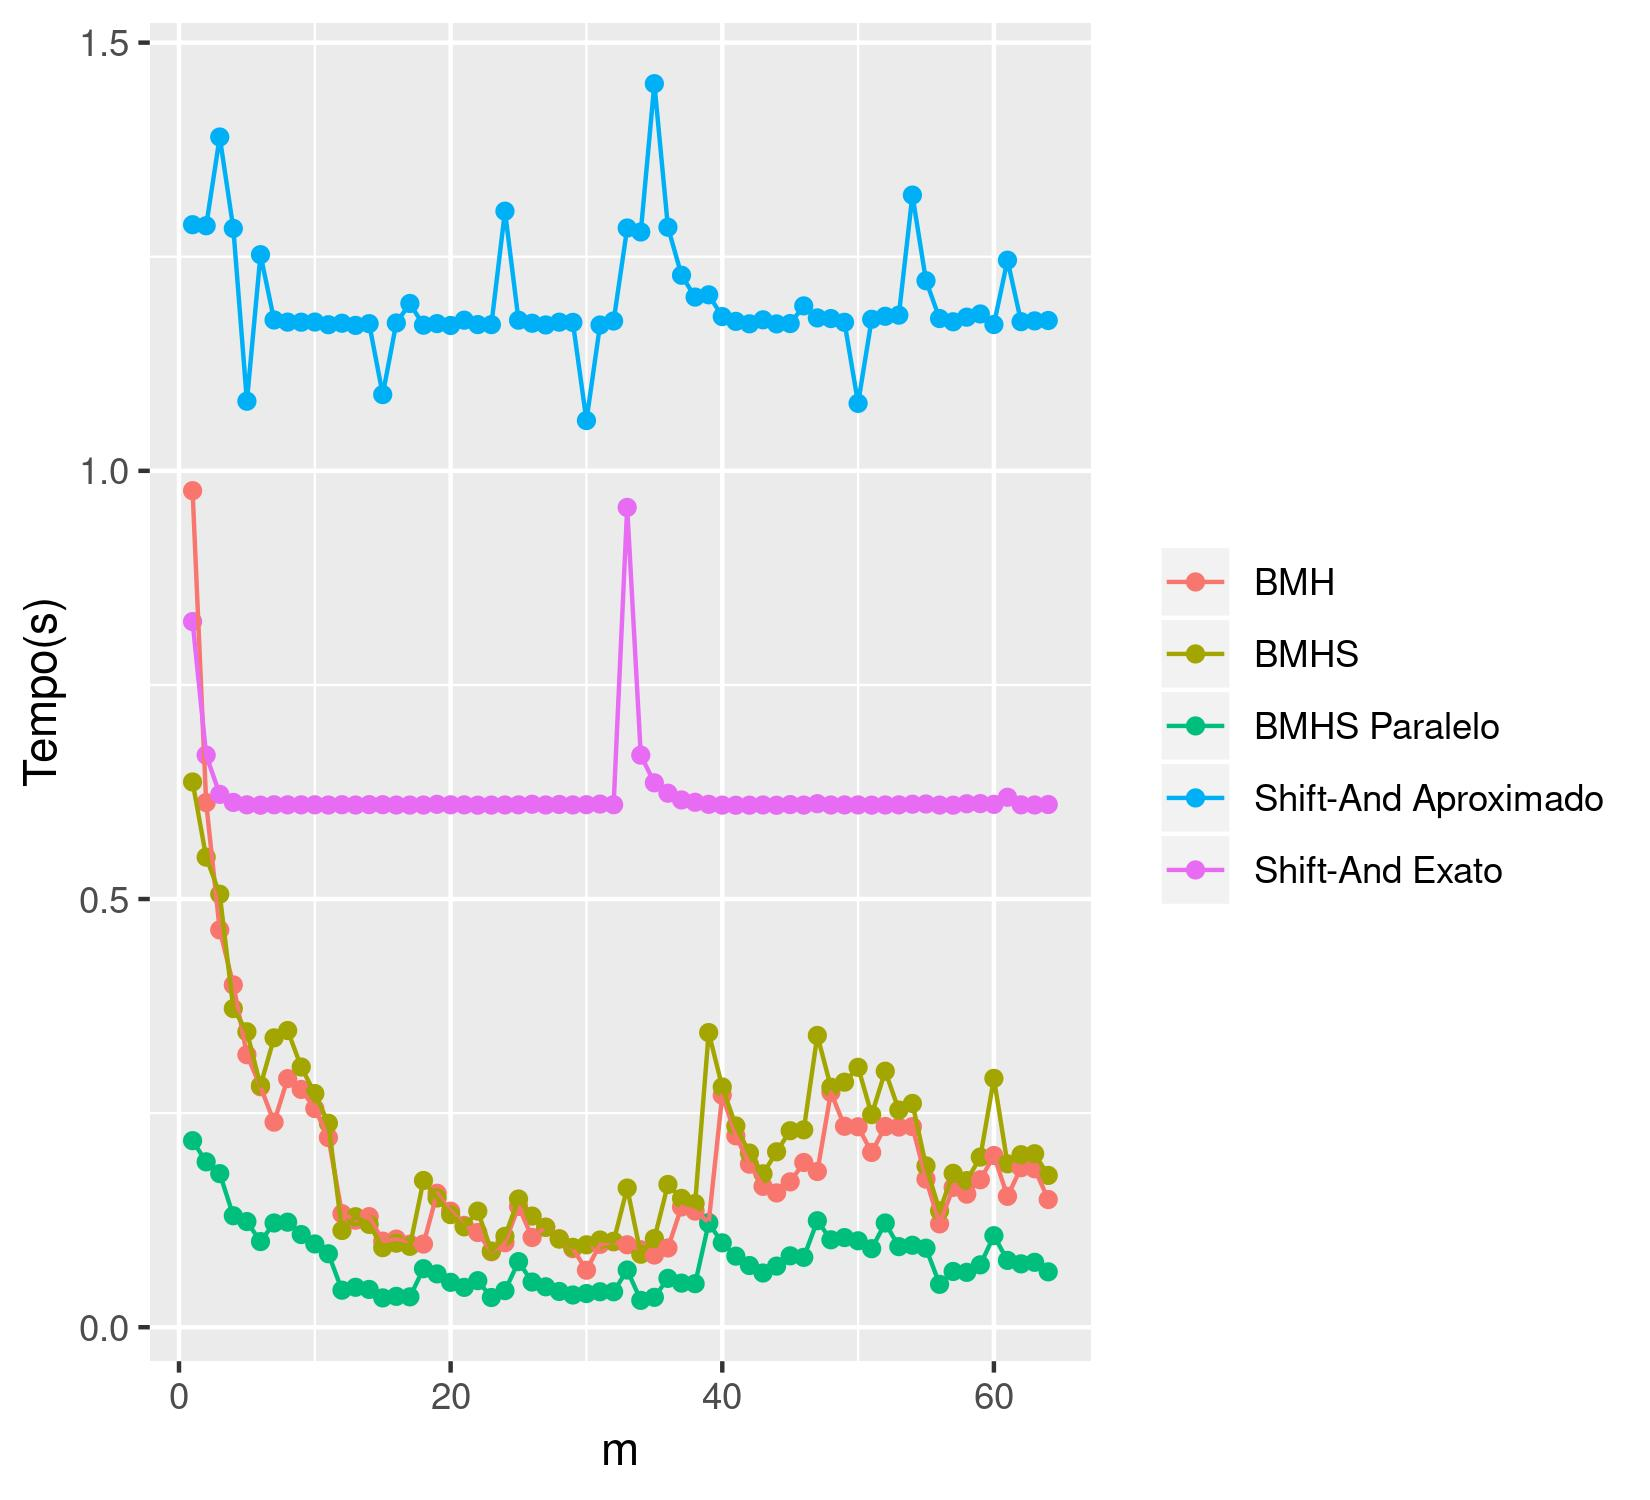
\includegraphics[width=4.5cm]{mxtimewordbound}
\caption{$m\leq \beta$.}\label{fig:mxtimewordbound}
\end{subfigure}
\begin{subfigure}[b]{.49\linewidth}
\centering
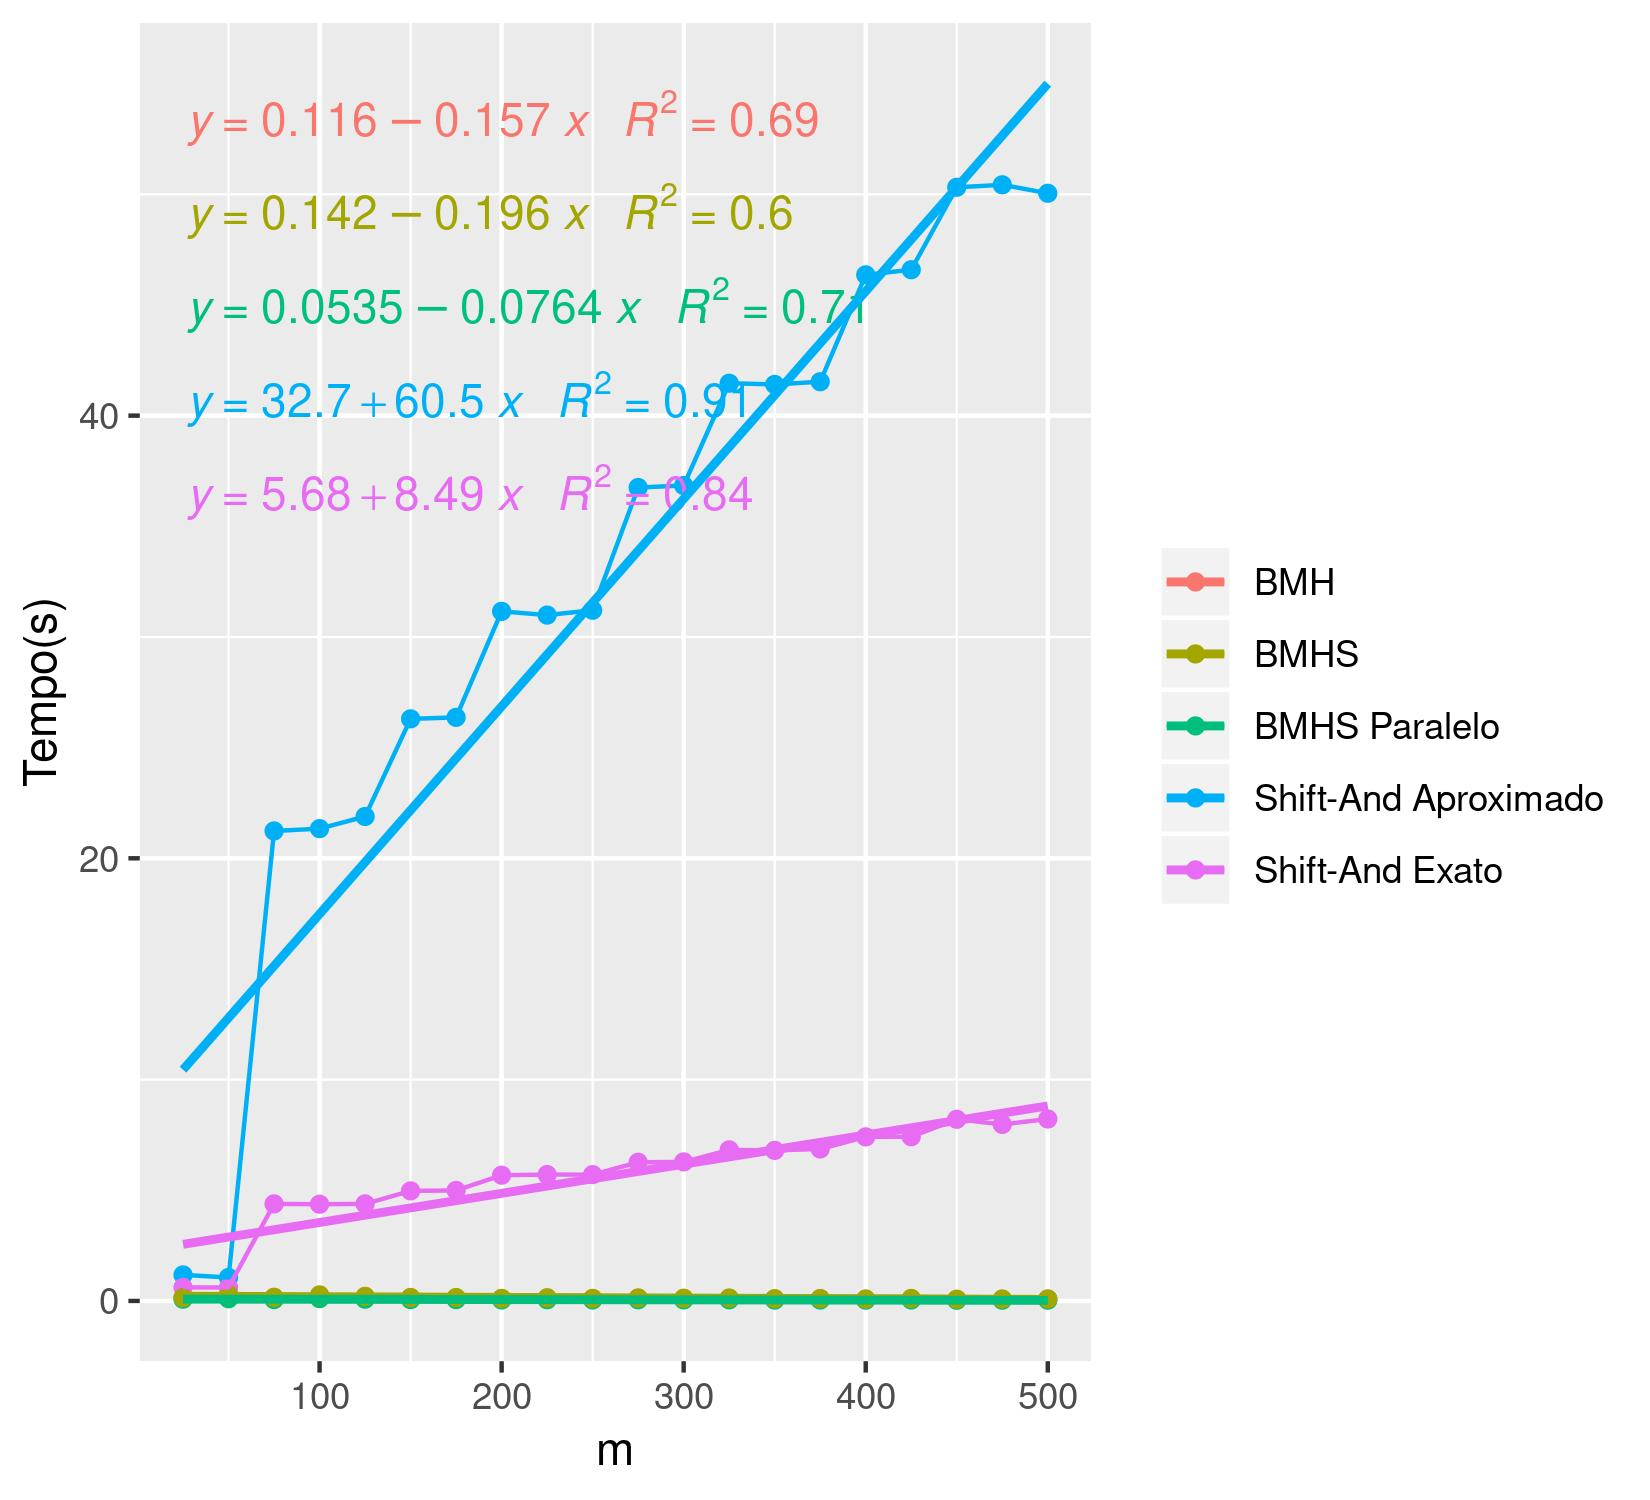
\includegraphics[width=4.5cm]{mxtimenobound}
\caption{m sem limite.}\label{fig:mxtimenobound}
\end{subfigure}
\caption{Tempo de acordo com tamanho do padrão na base $\iota$.}
\end{figure}
\end{center}

\begin{wrapfigure}{R}{5.5cm}
\caption{Base $\iota$.}\label{fig:mxtimenoboundb}
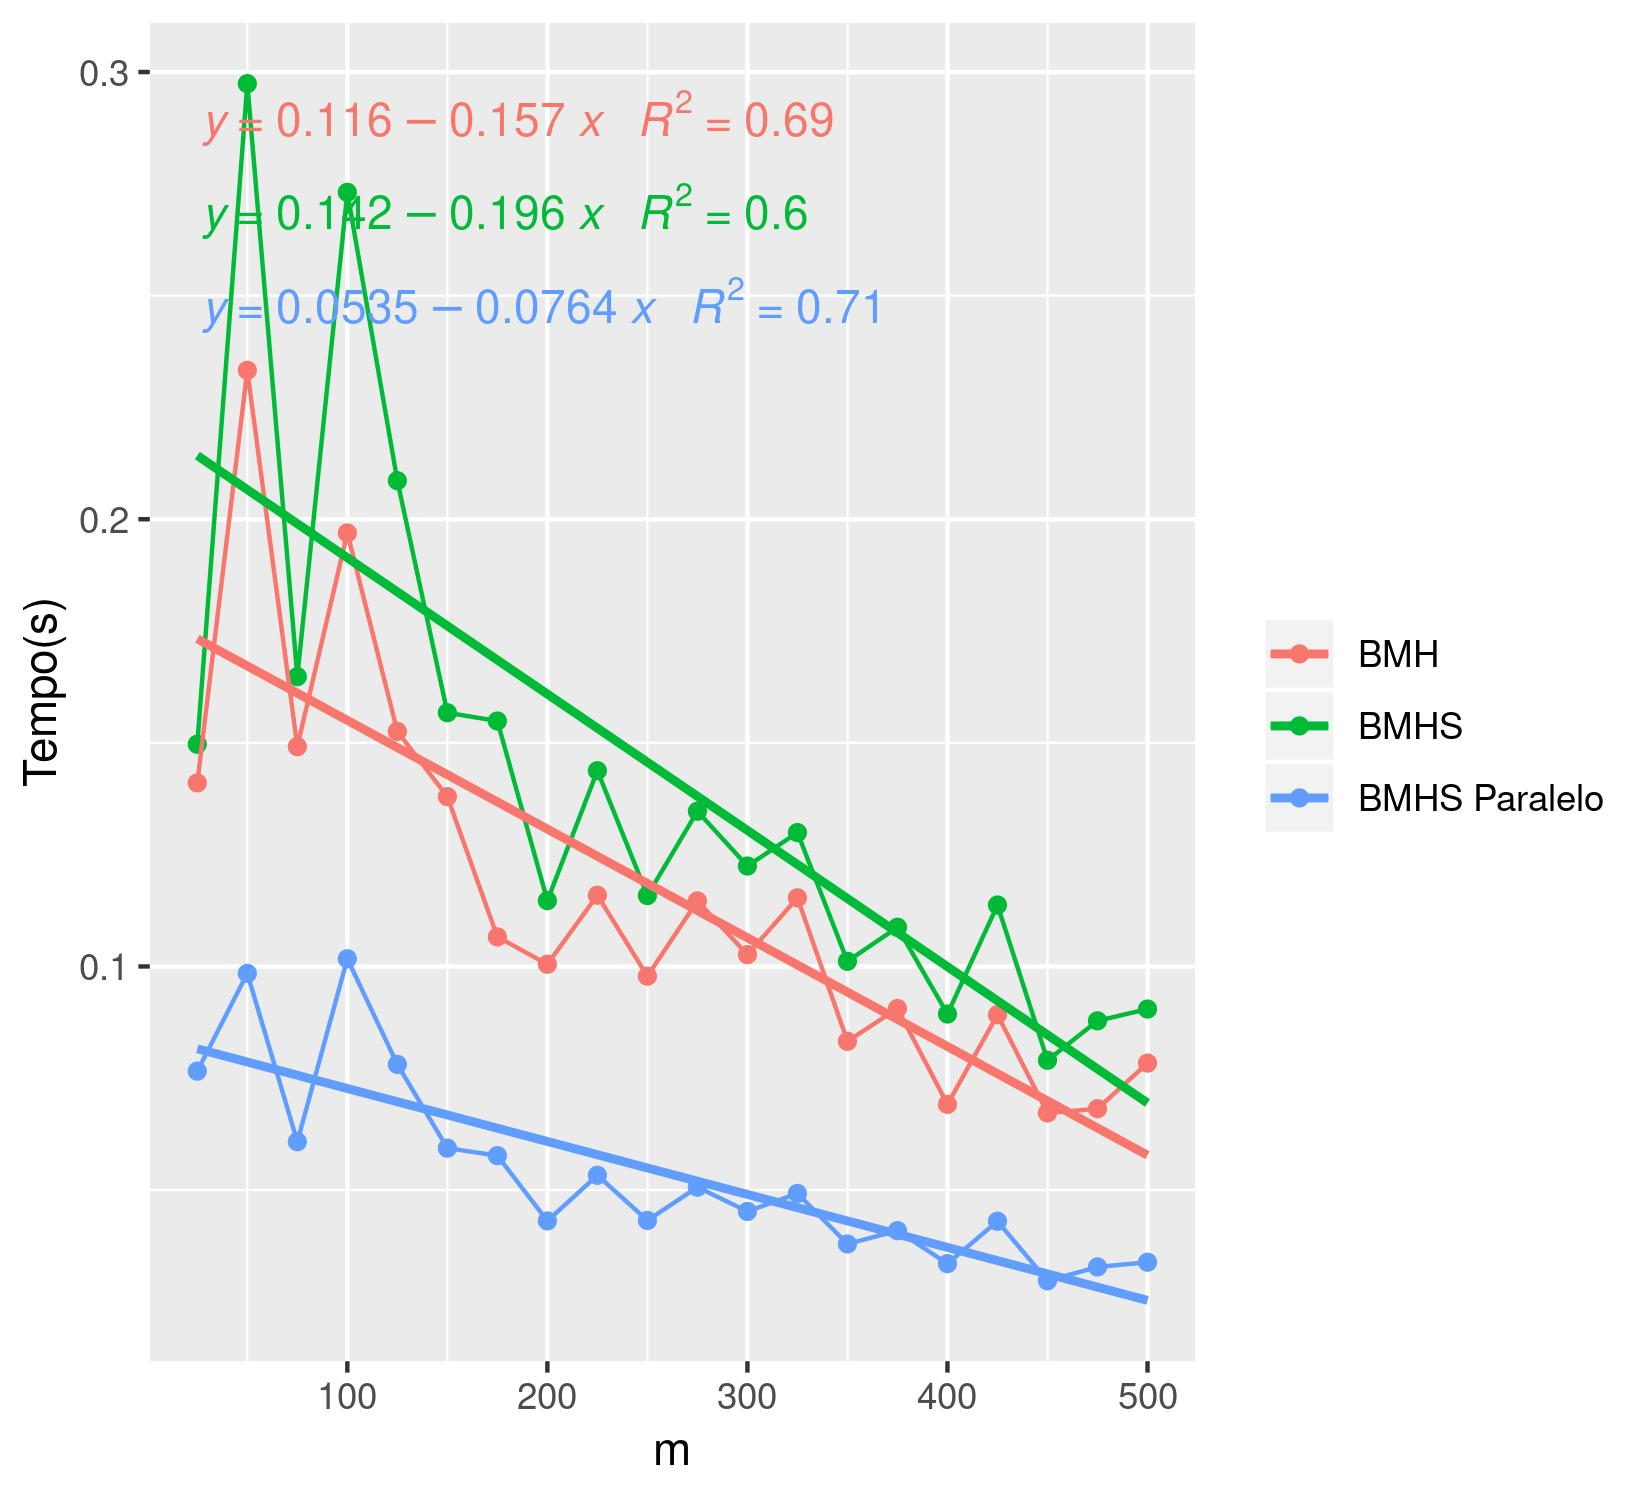
\includegraphics[width=5.5cm]{mxtimenoboundb}
\end{wrapfigure} 

\begin{center}
\begin{figure}
\begin{subfigure}[b]{.49\linewidth}
\centering
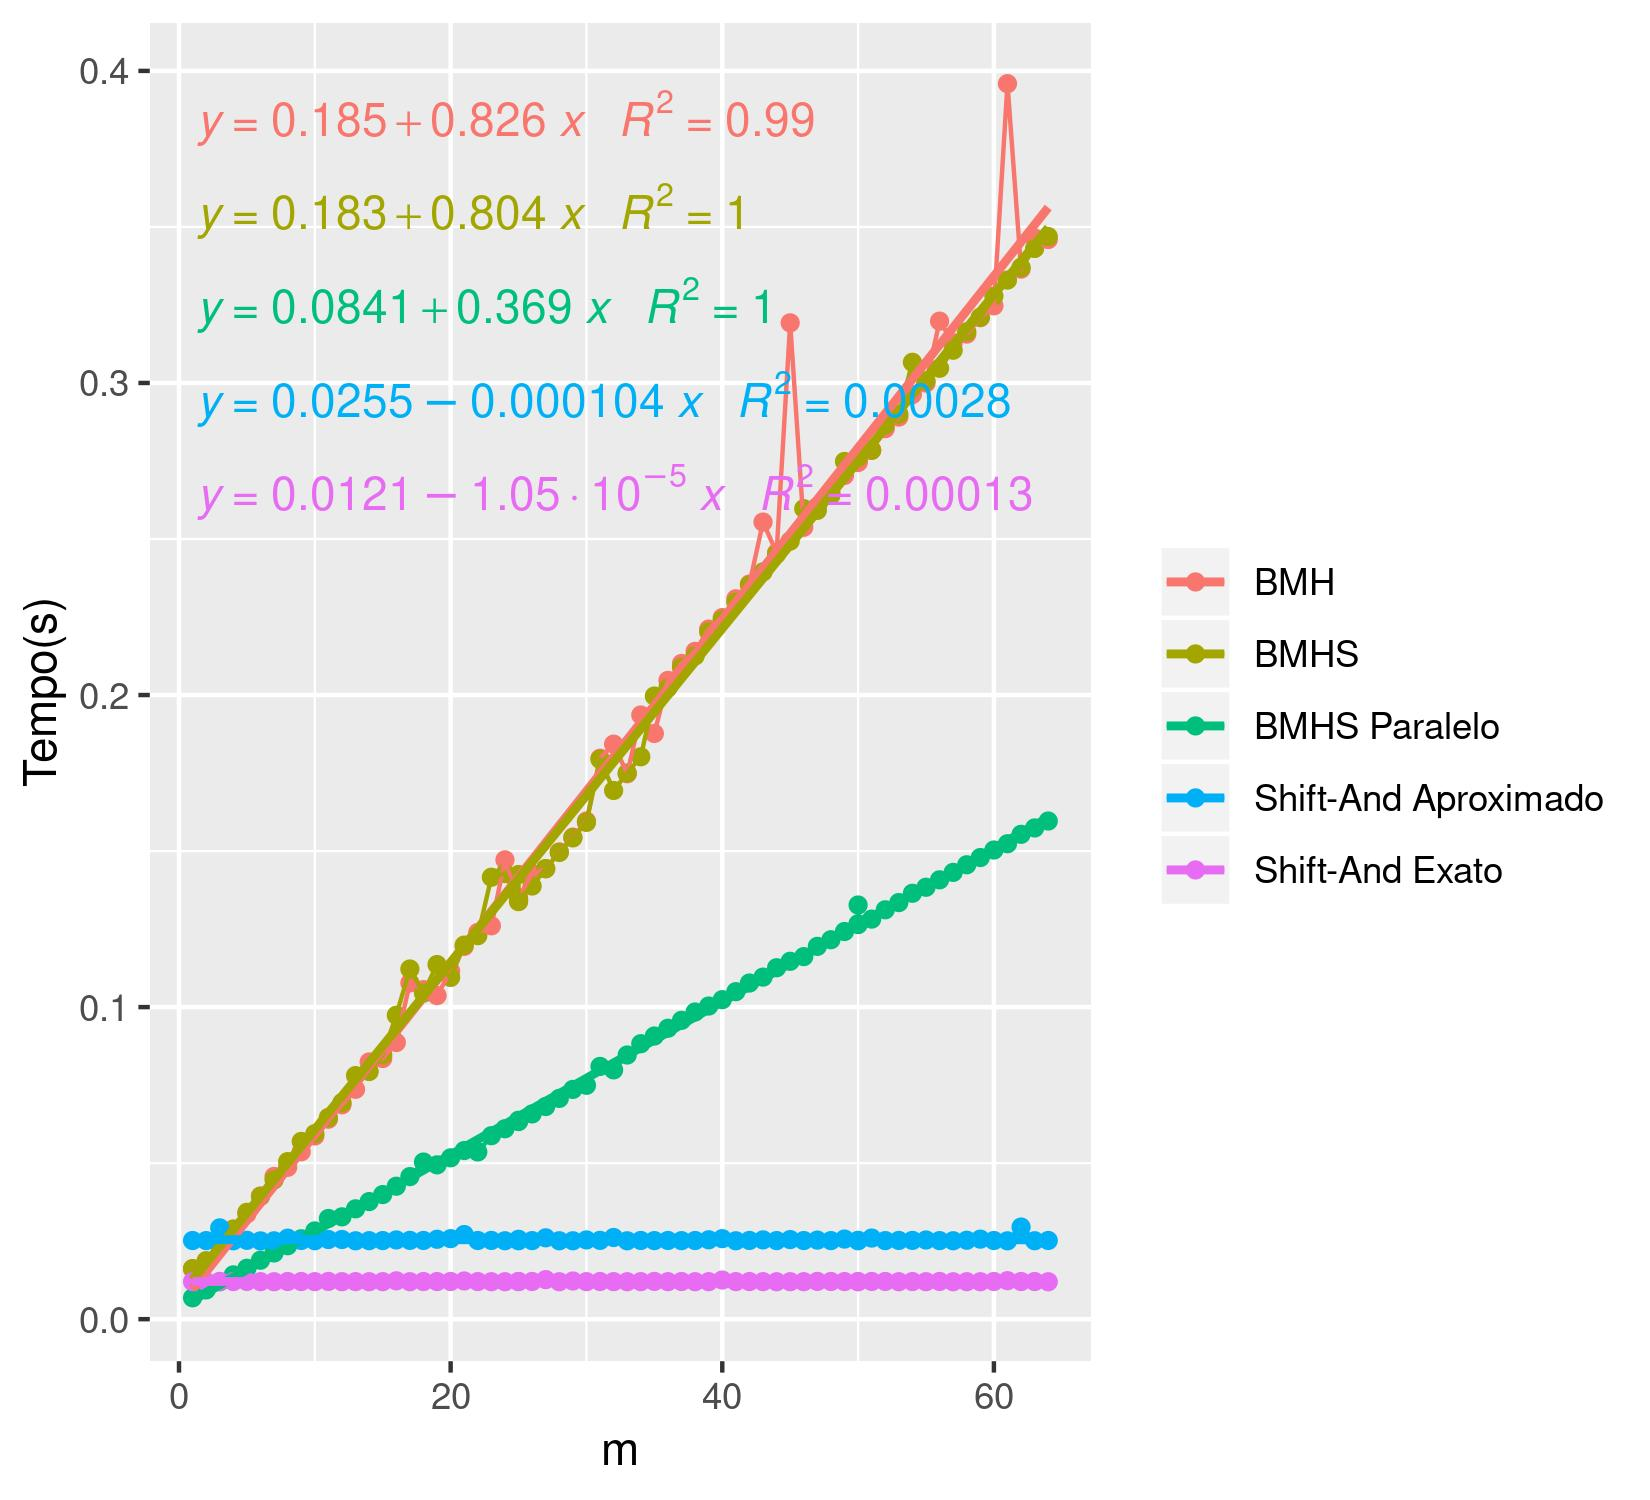
\includegraphics[width=4.5cm]{mxtimewordboundworst}
\caption{$m\leq \beta$.}\label{fig:mxtimewordboundworst}
\end{subfigure}
\begin{subfigure}[b]{.49\linewidth}
\centering
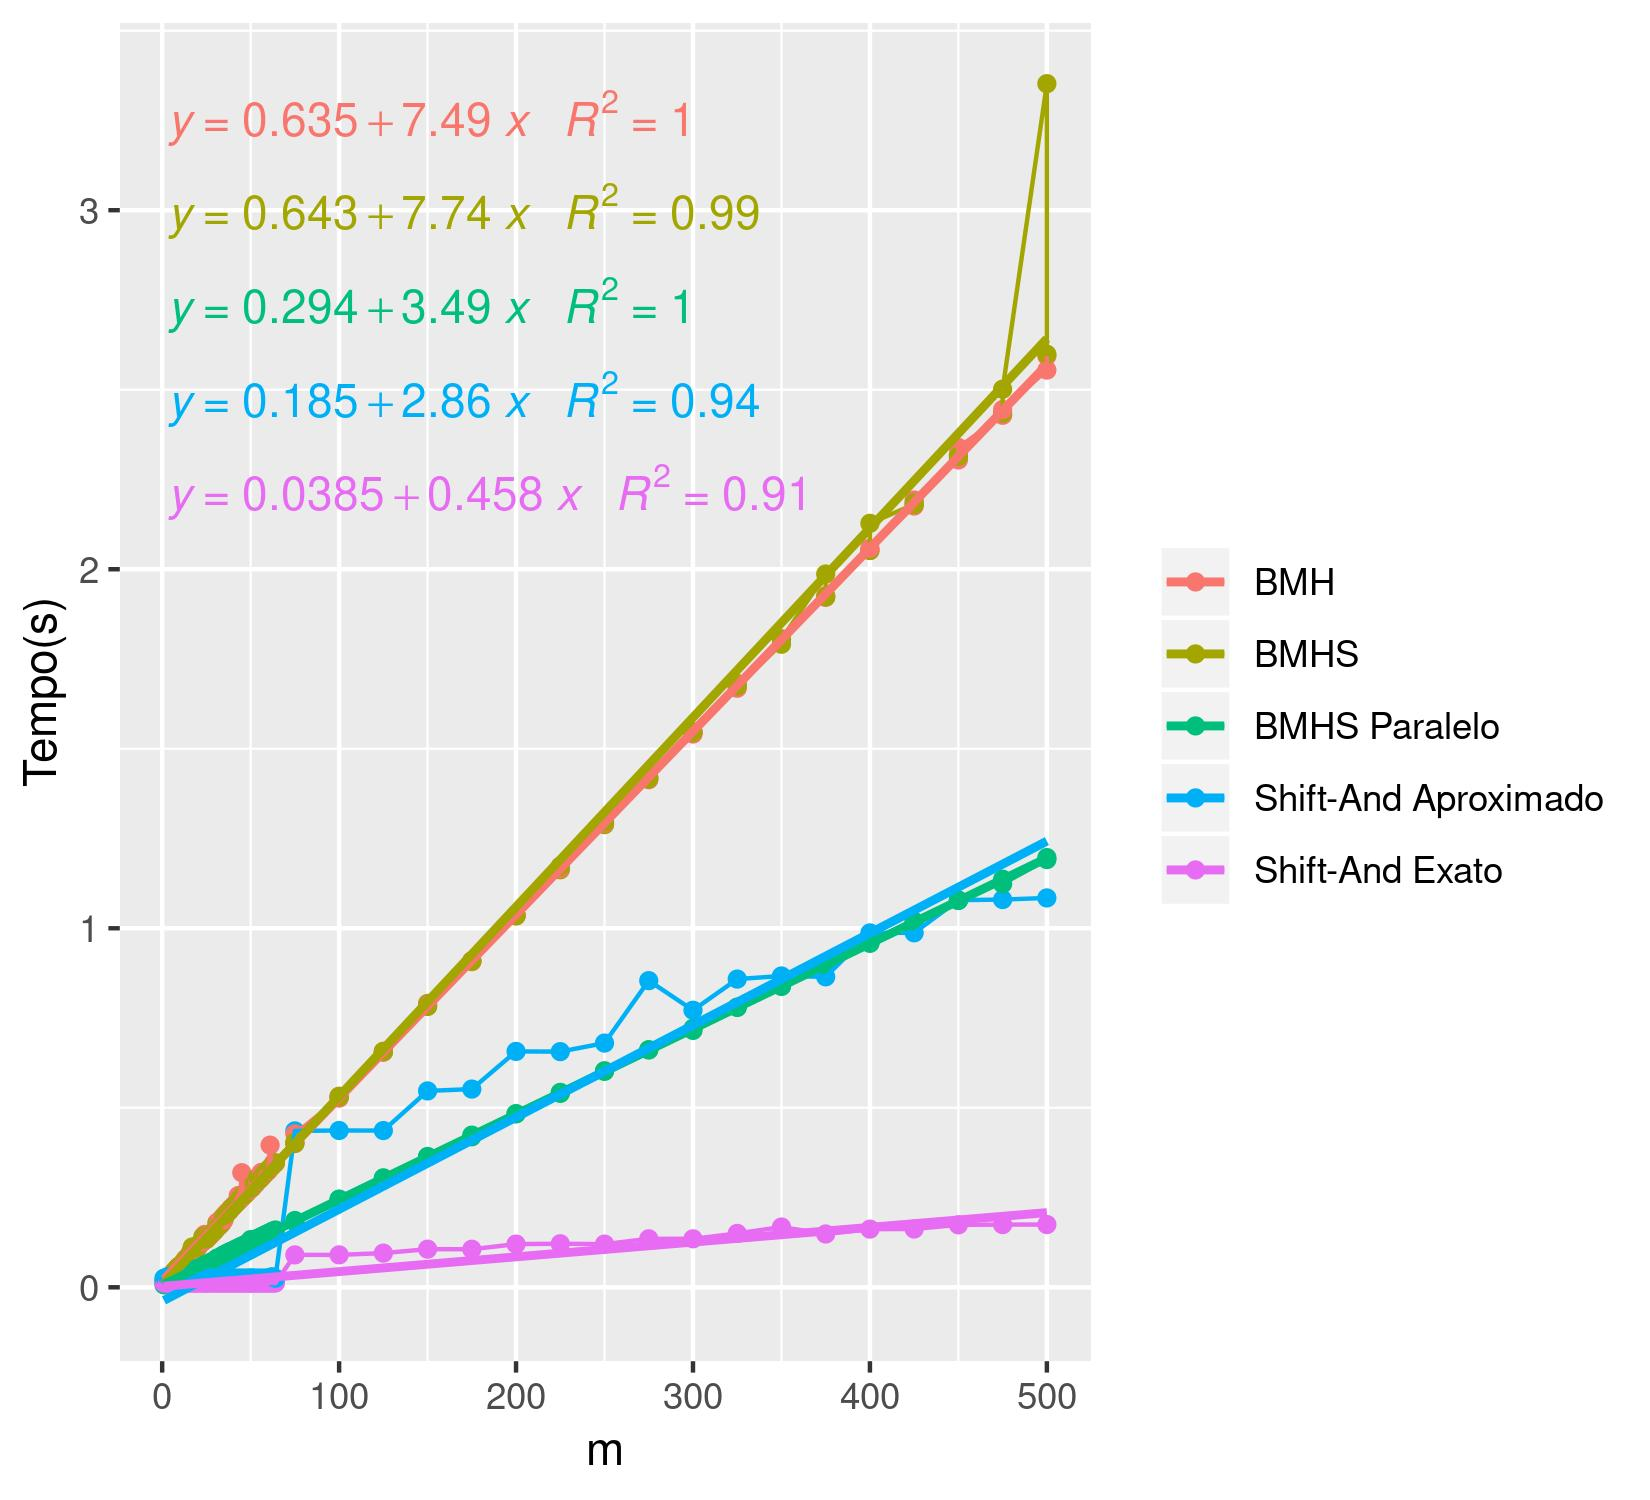
\includegraphics[width=4.5cm]{mxtimenoboundworst}
\caption{m sem limite.}\label{fig:mxtimenoboundworst}
\end{subfigure}
\caption{Tempo de acordo com tamanho do padrão na base A, pior caso.}\label{fig:mxtimeworstg}
\end{figure}
\end{center}

\subsubsection{Tamanho do texto (n)}
\label{sec:orgb07aaf8}
O próximo passo é analisar e comprovar a influência do tamanho do texto \(T\) nos algoritmos.

A figura \ref{fig:nxtime} mostra o crescimento do tempo de acordo com o tamanho do arquivo. O gráfico mostra que há um crescimento linear do tempo de acordo com o tamanho do arquivo para todos algoritmos, assim comprovando uma parte da complexidade obtida.

A figura \ref{fig:nxcomp} mostra o crescimento das comparações. Os números de comparações formam um gráfico similar ao gráfico com tempo, assim reforçando que o gráfico obtido com tempo é correto. Esses gráficos reforçam a inferioridade do Shift-And para casos médios, basta observar a diferença do número de comparações de qualquer um dos outros algoritmos.



\begin{figure}
\begin{subfigure}[b]{.49\linewidth}
\centering
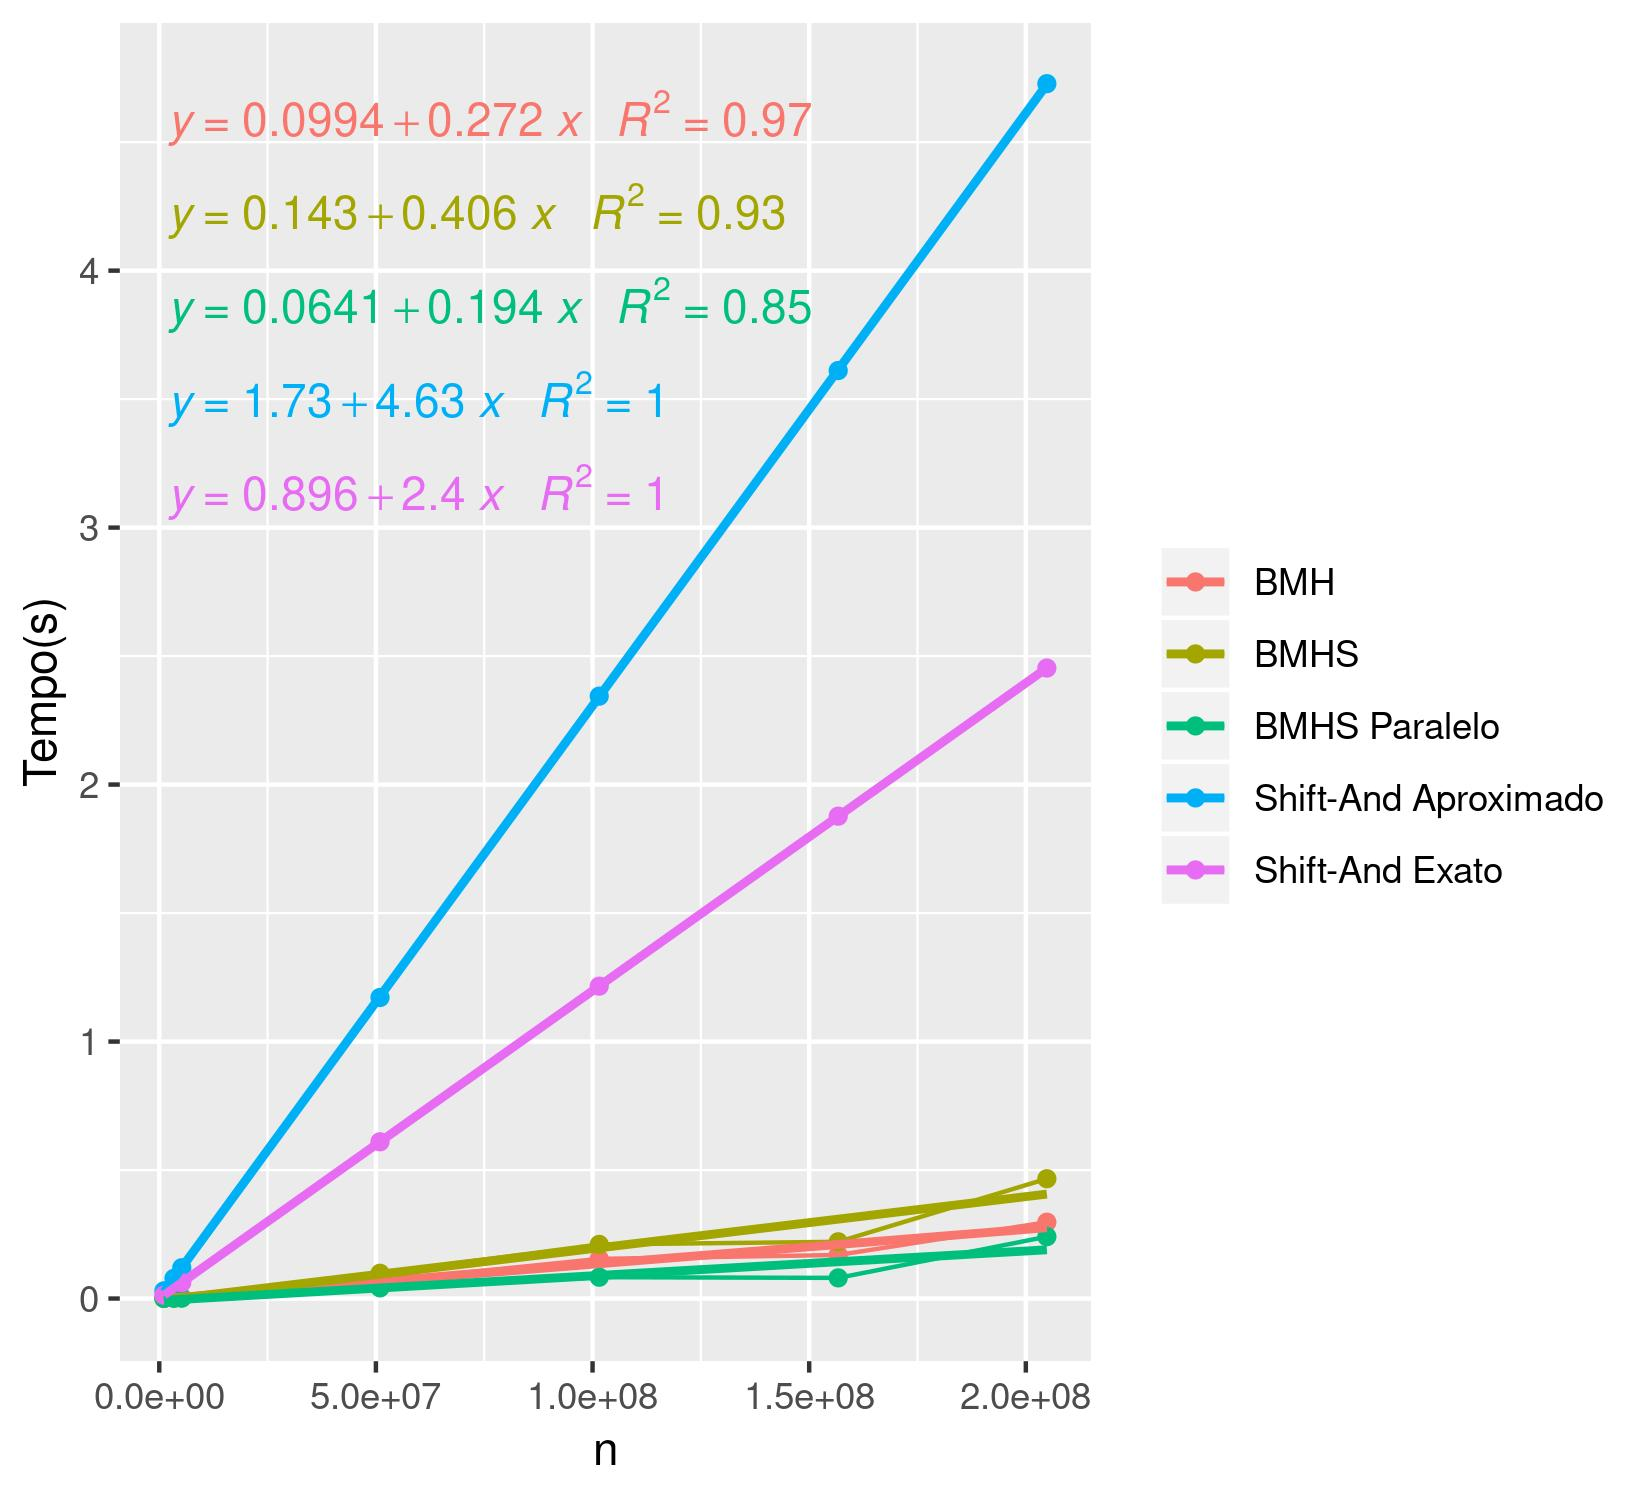
\includegraphics[width=7.5cm]{nxtime}
\caption{}\label{fig:nxtime}
\end{subfigure}
\begin{subfigure}[b]{.49\linewidth}
\centering
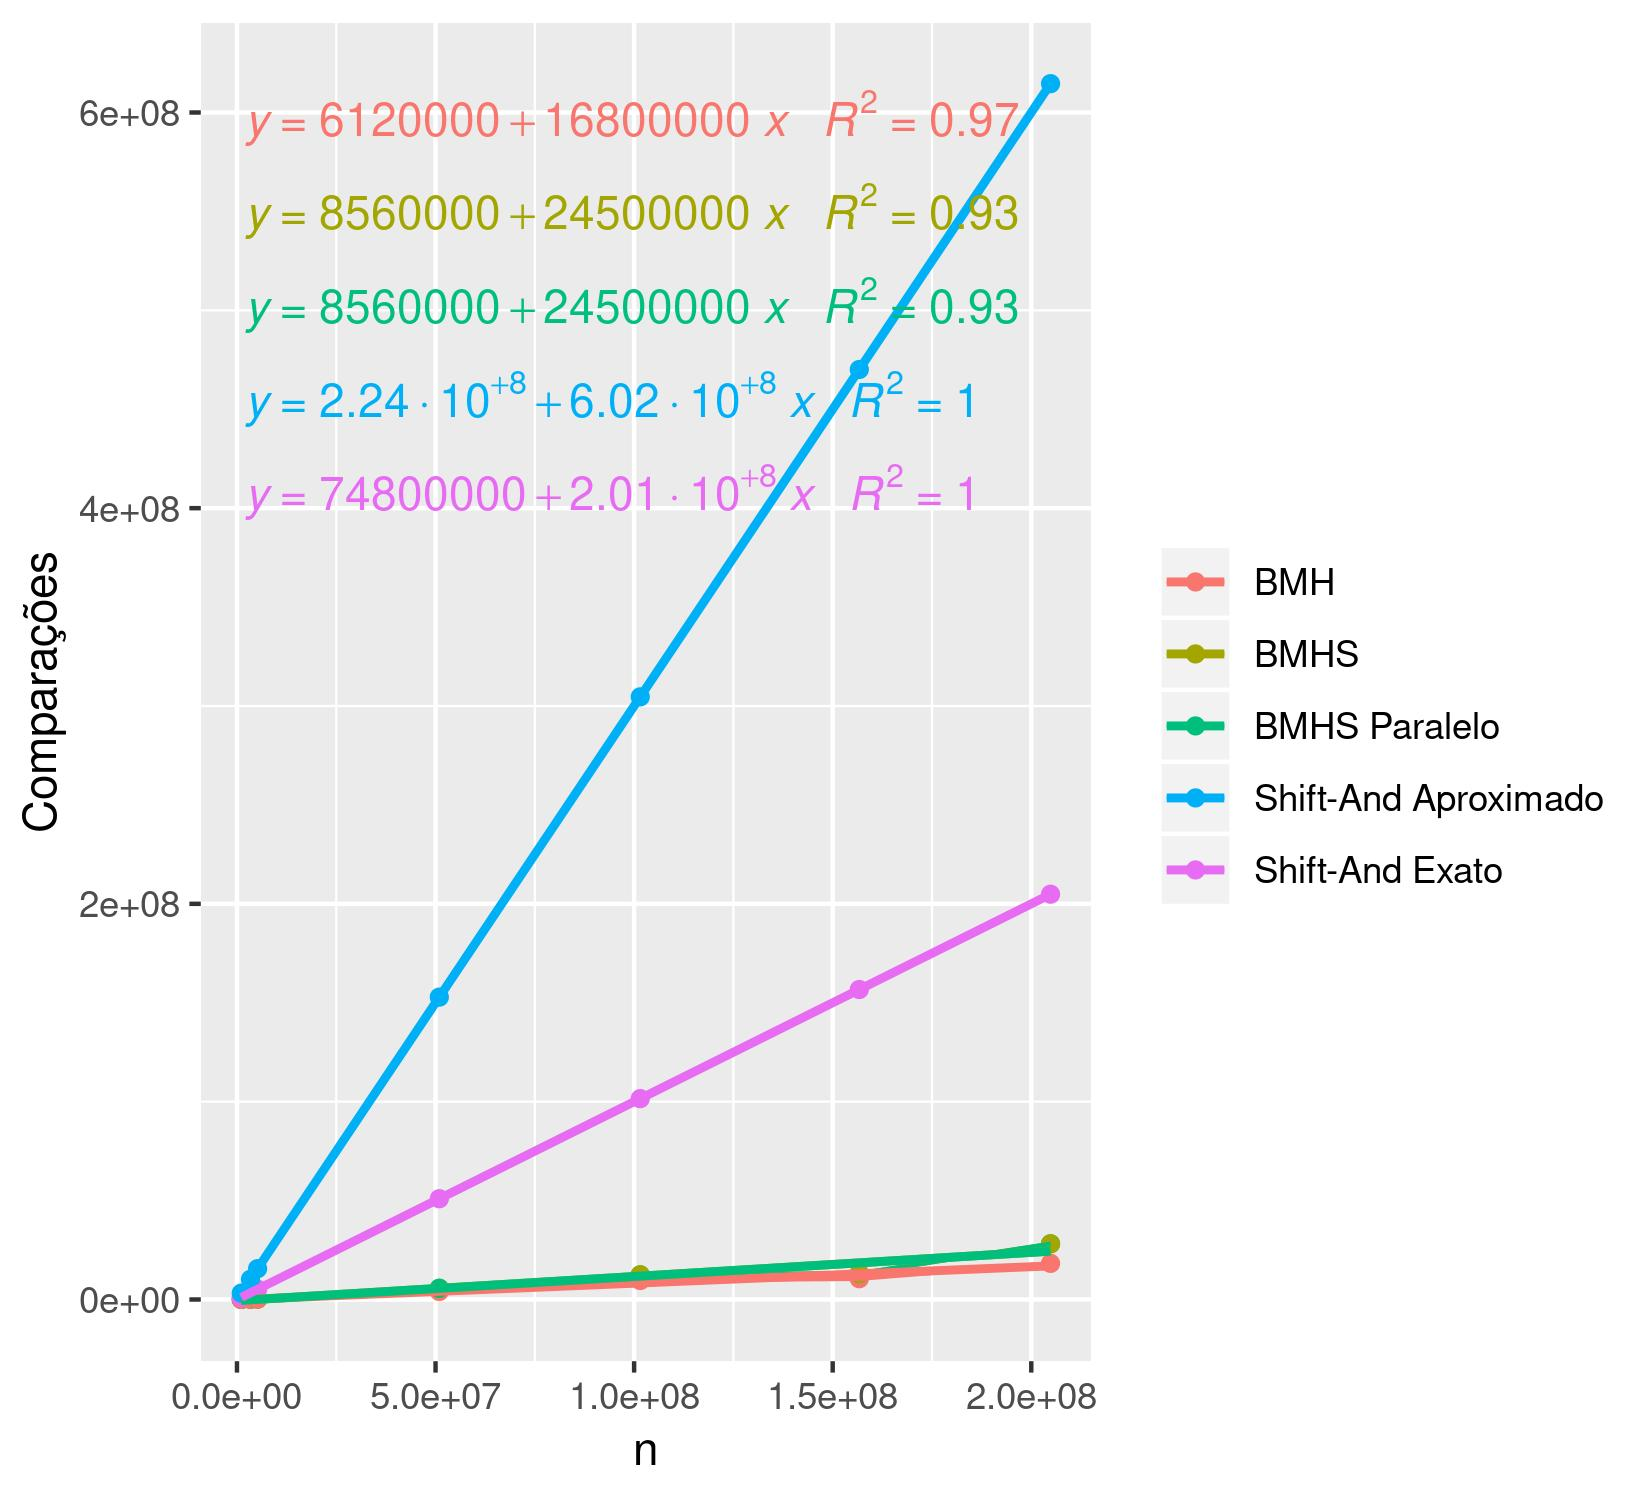
\includegraphics[width=7.5cm]{nxcomp}
\caption{}\label{fig:nxcomp}
\end{subfigure}
\caption{Variação de n com todas bases exceto A e m=30.}\label{fig:nxg}
\end{figure}

\subsubsection{Erro(error)}
\label{sec:org4f1a0a0}
Agora é necessário avaliar o impacto do número de erros no tempo de execução. A figura \ref{fig:errorxtime} mostra o comportamento, o tempo cresce linearmente como previsto logo foi comprovado o termo de erro na complexidade tempo do algoritmo ShiftAnd.

\begin{wrapfigure}{R}{4.3cm}
\caption{m=30,base=$\iota$,Shift-And aproximado}\label{fig:errorxtime}
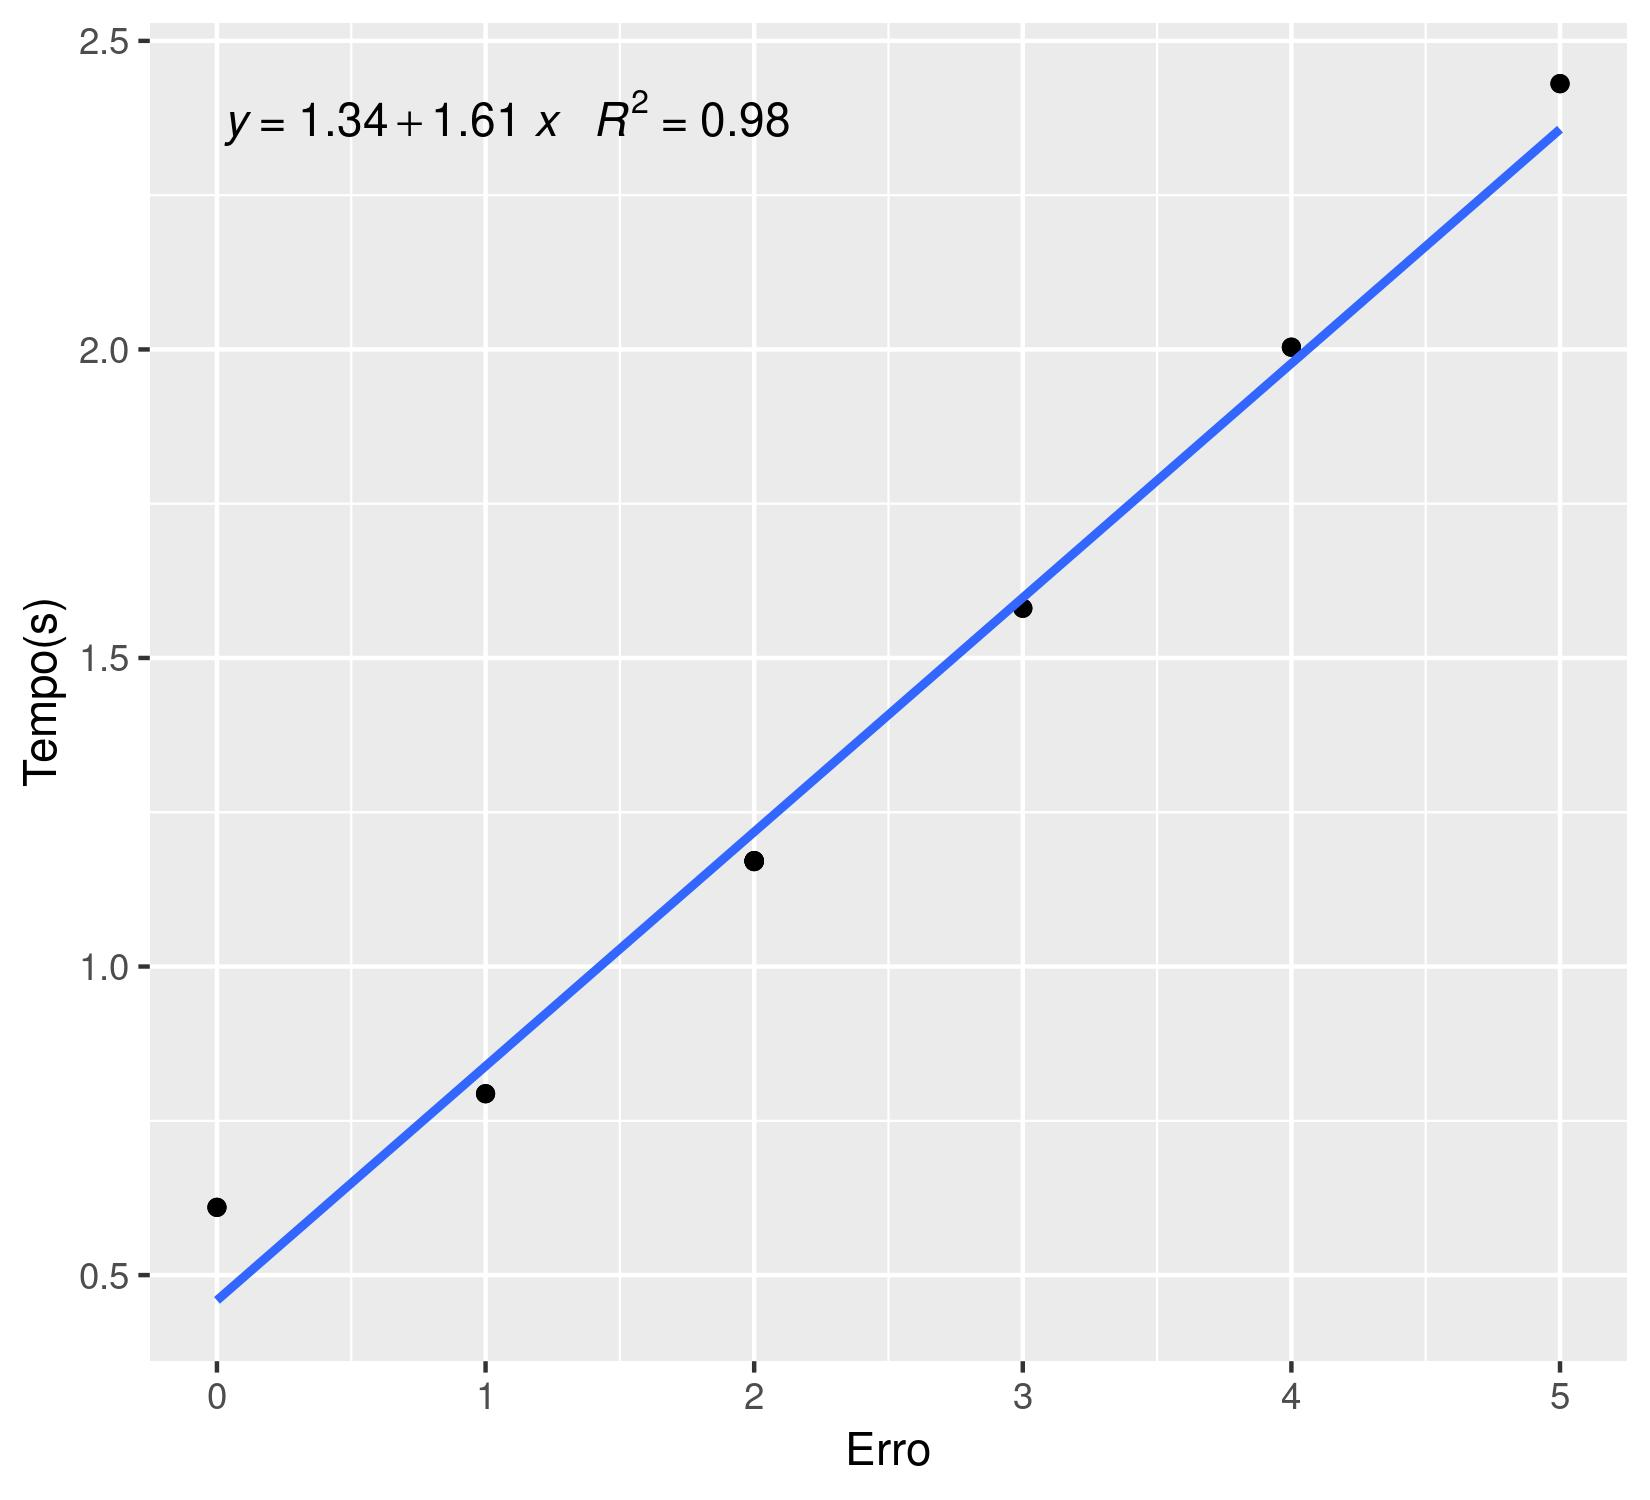
\includegraphics[width=4.3cm]{errorxtime}
\end{wrapfigure} 

\subsubsection{Processadores(p)}
\label{sec:org2badbbd}

Agora basta analisar o comportamento do algoritmo BMHS paralelo com o crescimento do número de processadores. Primeiro é importante definir alguns termos para ser feito a avaliação. O primeiro deles é o speedup que é igual a \(S=\frac{\text{Tempo do algoritmo sequencial usando 1 processador}}{\text{Tempo do algoritmo paralelo usando p processadores}}\), o próximo termo é a eficiência que será igual a \(E=\frac{S}{p}\), sendo p o número de processadores como já definido.

A figura \ref{fig:pxtime} mostra que de acordo com o aumento do número de processadores há um decaimento no tempo linearmente. Esse é o comportamento esperado que comprova o termo \(p\) na complexidade de tempo do algoritmo BMHS paralelo. 

Após isso basta avaliar o speedup obtido com a implementação feita. A figura \ref{fig:mxspeedup} mostra o speedup na base \(\iota\) com 4 processadores, esse speedup não foi perfeito porém esta bem próximo, na média sendo \(S_{4}\approx 3.18\), porém é importante notar que na figura os valores de m pequenos tiveram um speedup menor, já para grandes valores de m o algoritmo se estabilizou numa média um pouco melhor. Porém já para 2 processadores, como mostra na figura \ref{fig:mxspeedup2p}, o speedup é na média \(S_{2}\approx 1.78\).

A figura \ref{fig:nxspeedup} mostra o speedup de acordo com a base usada. Os resultados obtidos foram parecidos com a variação de \(m\) na base \(\iota\).

Então de acordo com os dados obtidos a eficiência é \(E_{4}\approx 0.795\) para 4 processadores e para 2 processadores é \(E_{2}\approx 0.89\). A eficiência é significativamente maior com 2 processadores como pode ser observado.

Outro fator importante que pode impactar o desempenho do algoritmo é o número de comparações que existe de diferença entre o BMHS paralelo e BMHS serial. A figura \ref{fig:mxcompparalelo} mostra que na média o BMHS paralelo tem aproximadamente 24 comparações a mais que o BMHS serial, esse valor é extremamente baixo visto que a média é de até um m igual a 5000. Logo esse valor mostra que o BMHS paralelo não sofre tantas consequências pela sua divisão de blocos. Também é importante notar que existe um crescimento do módulo do número de comparações junto com o crescimento de \(m\).

\begin{wrapfigure}{R}{4.5cm}
\caption{Tempo de acordo com número de processadores.}\label{fig:pxtime}
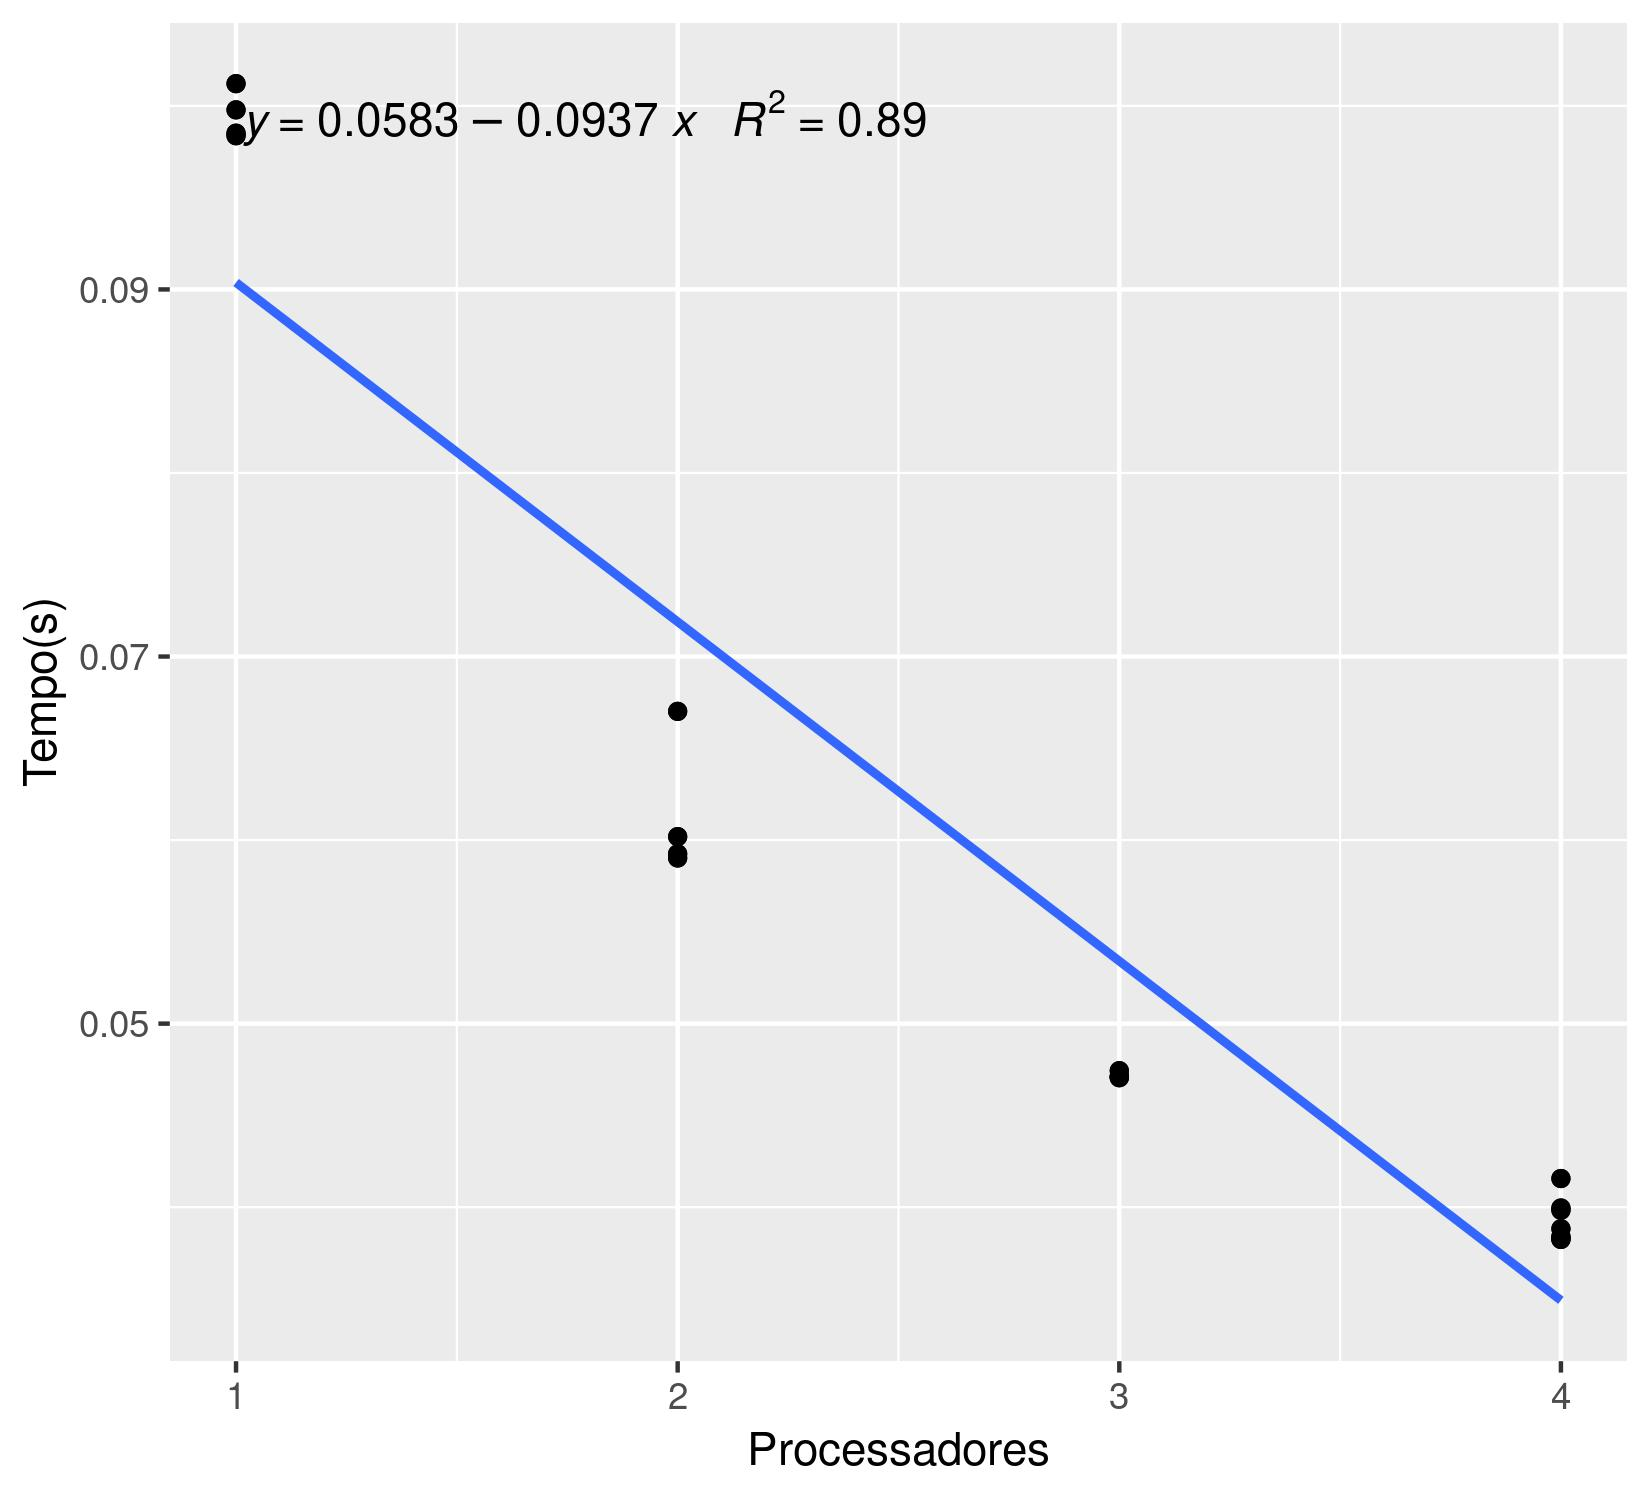
\includegraphics[width=4.5cm]{pxtime}
\end{wrapfigure} 
\begin{wrapfigure}{R}{5.5cm}
\end{wrapfigure}
\begin{wrapfigure}{R}{5.5cm}
\caption{Diferença de comparações BMHS serial e paralelo, base $\iota$.}\label{fig:mxcompparalelo}
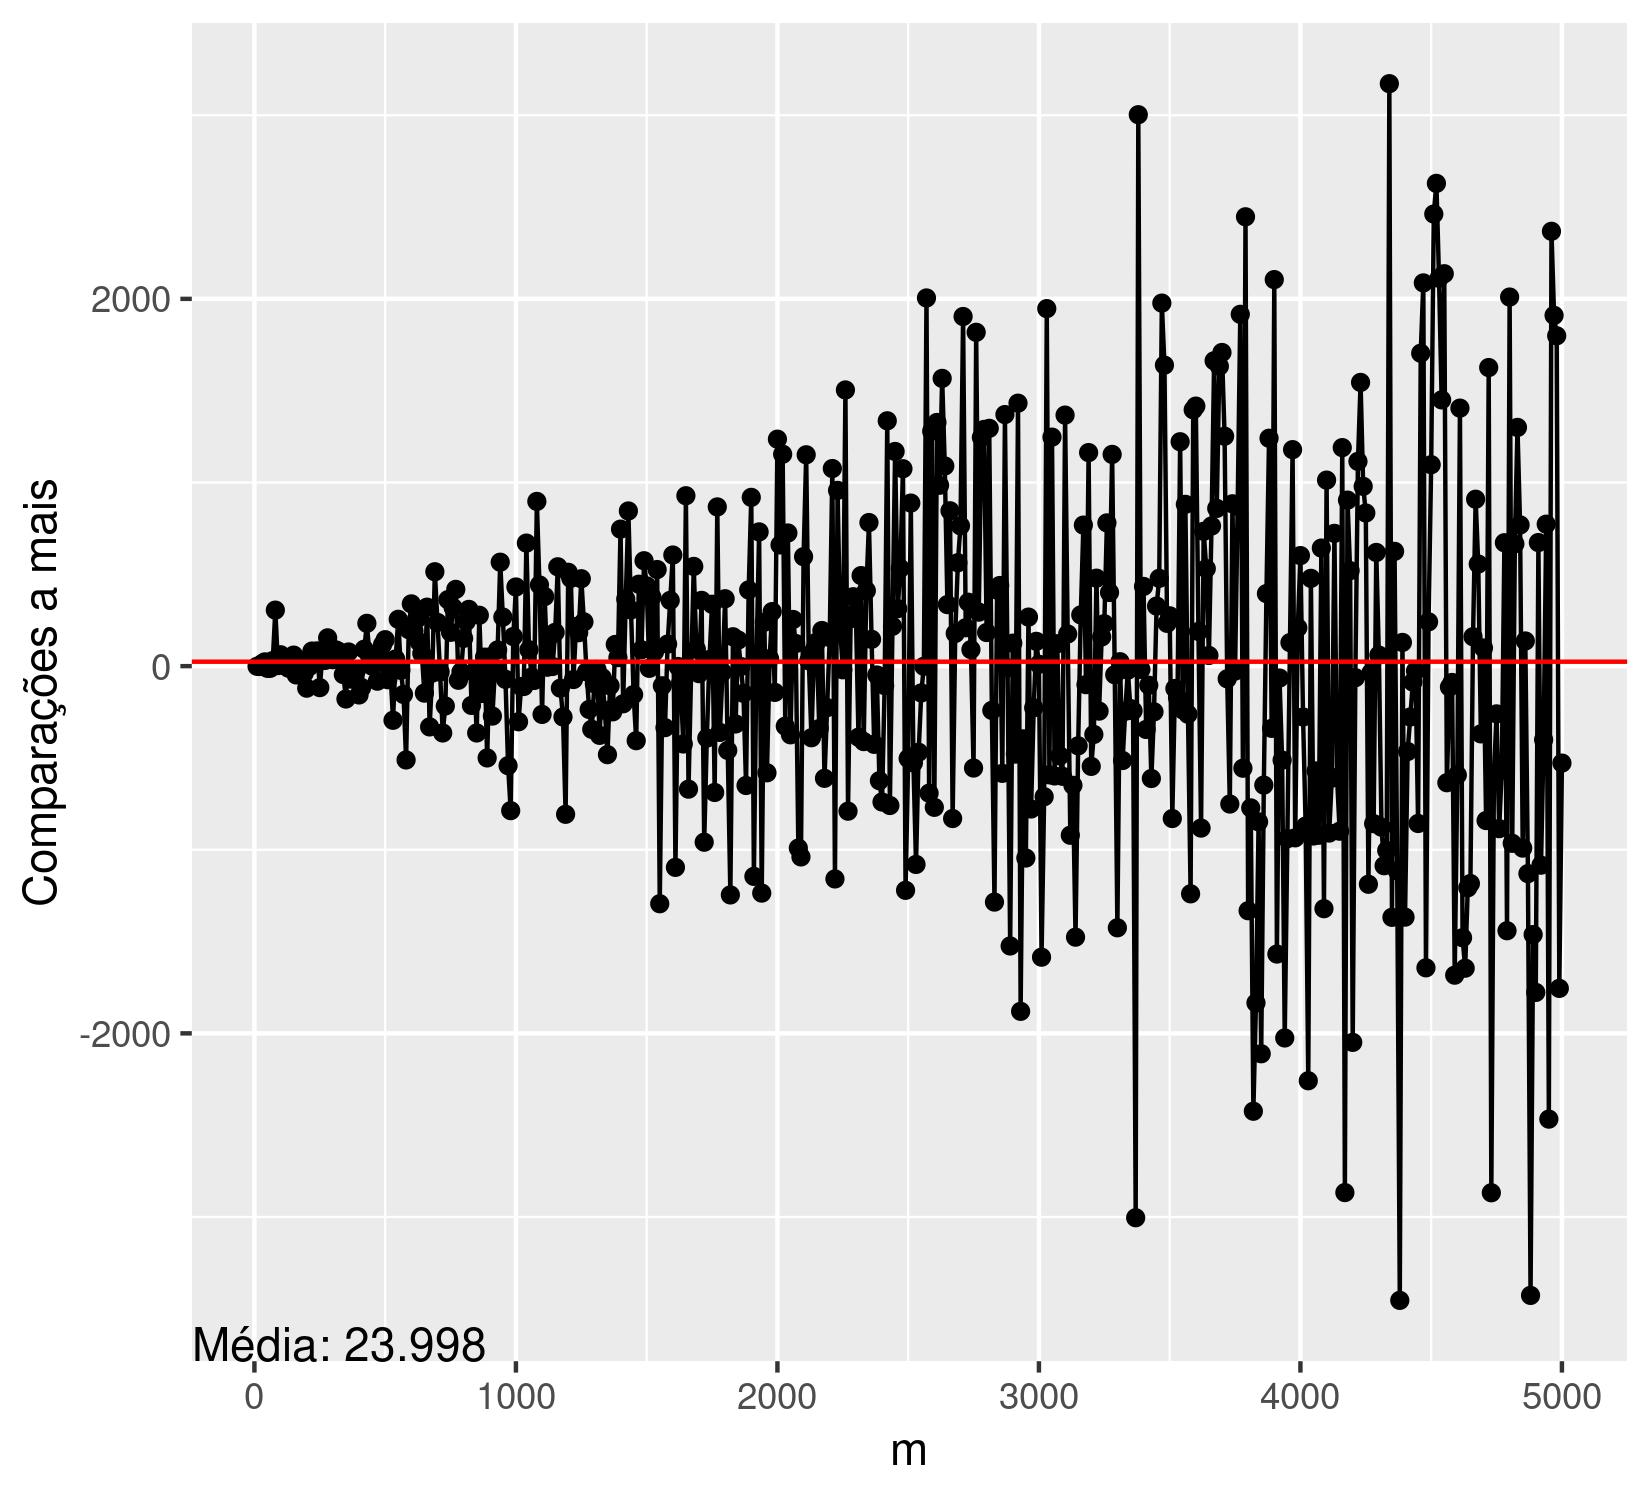
\includegraphics[width=5.5cm]{mxcompparalelo}
\end{wrapfigure}

\begin{center}
\begin{figure}
\begin{subfigure}[b]{.33\linewidth}
\centering
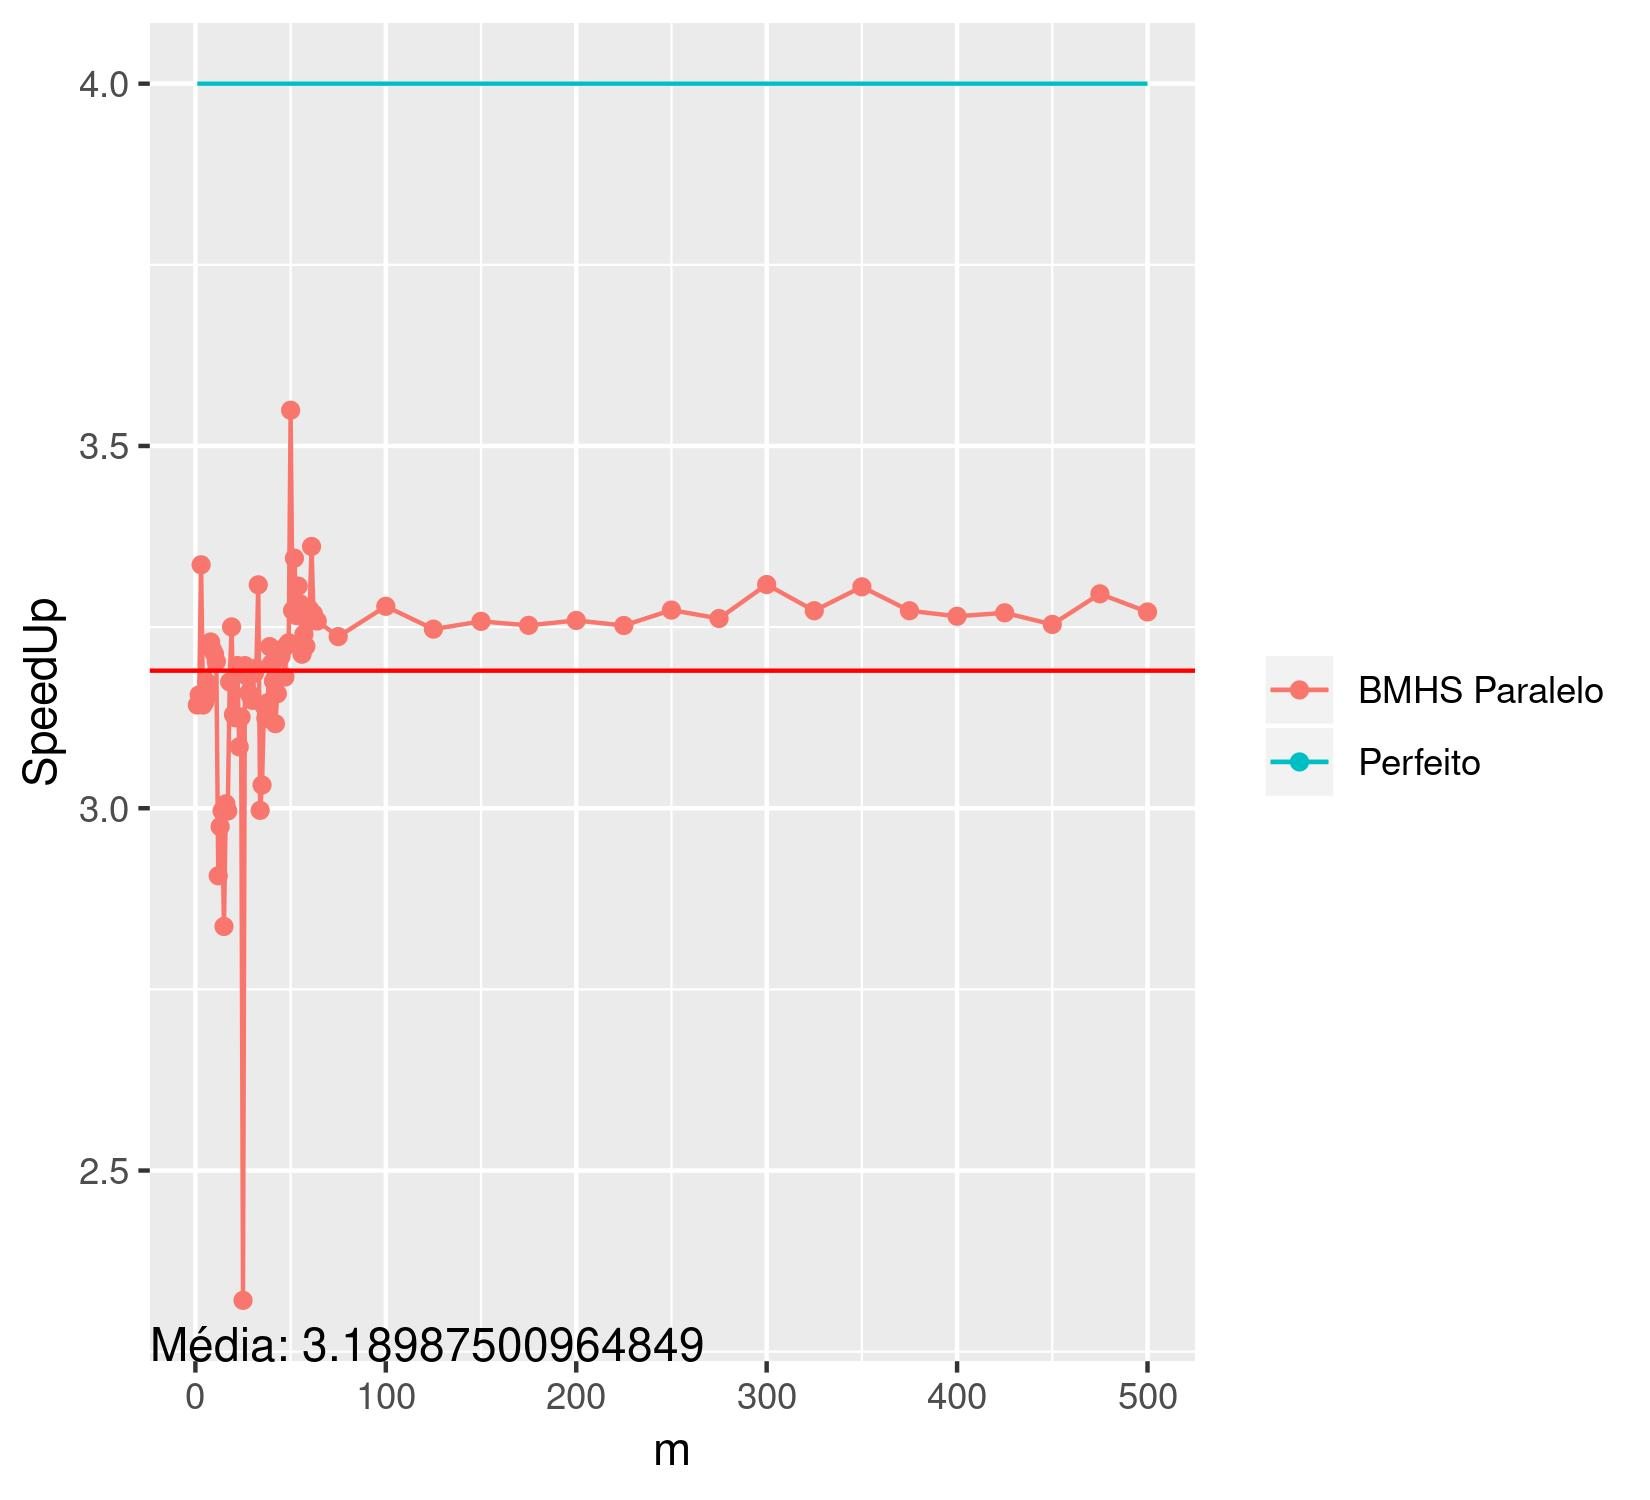
\includegraphics[width=5.5cm]{mxspeedup}
\caption{base=$\iota$,p=4}\label{fig:mxspeedup}
\end{subfigure}
\begin{subfigure}[b]{.33\linewidth}
\centering
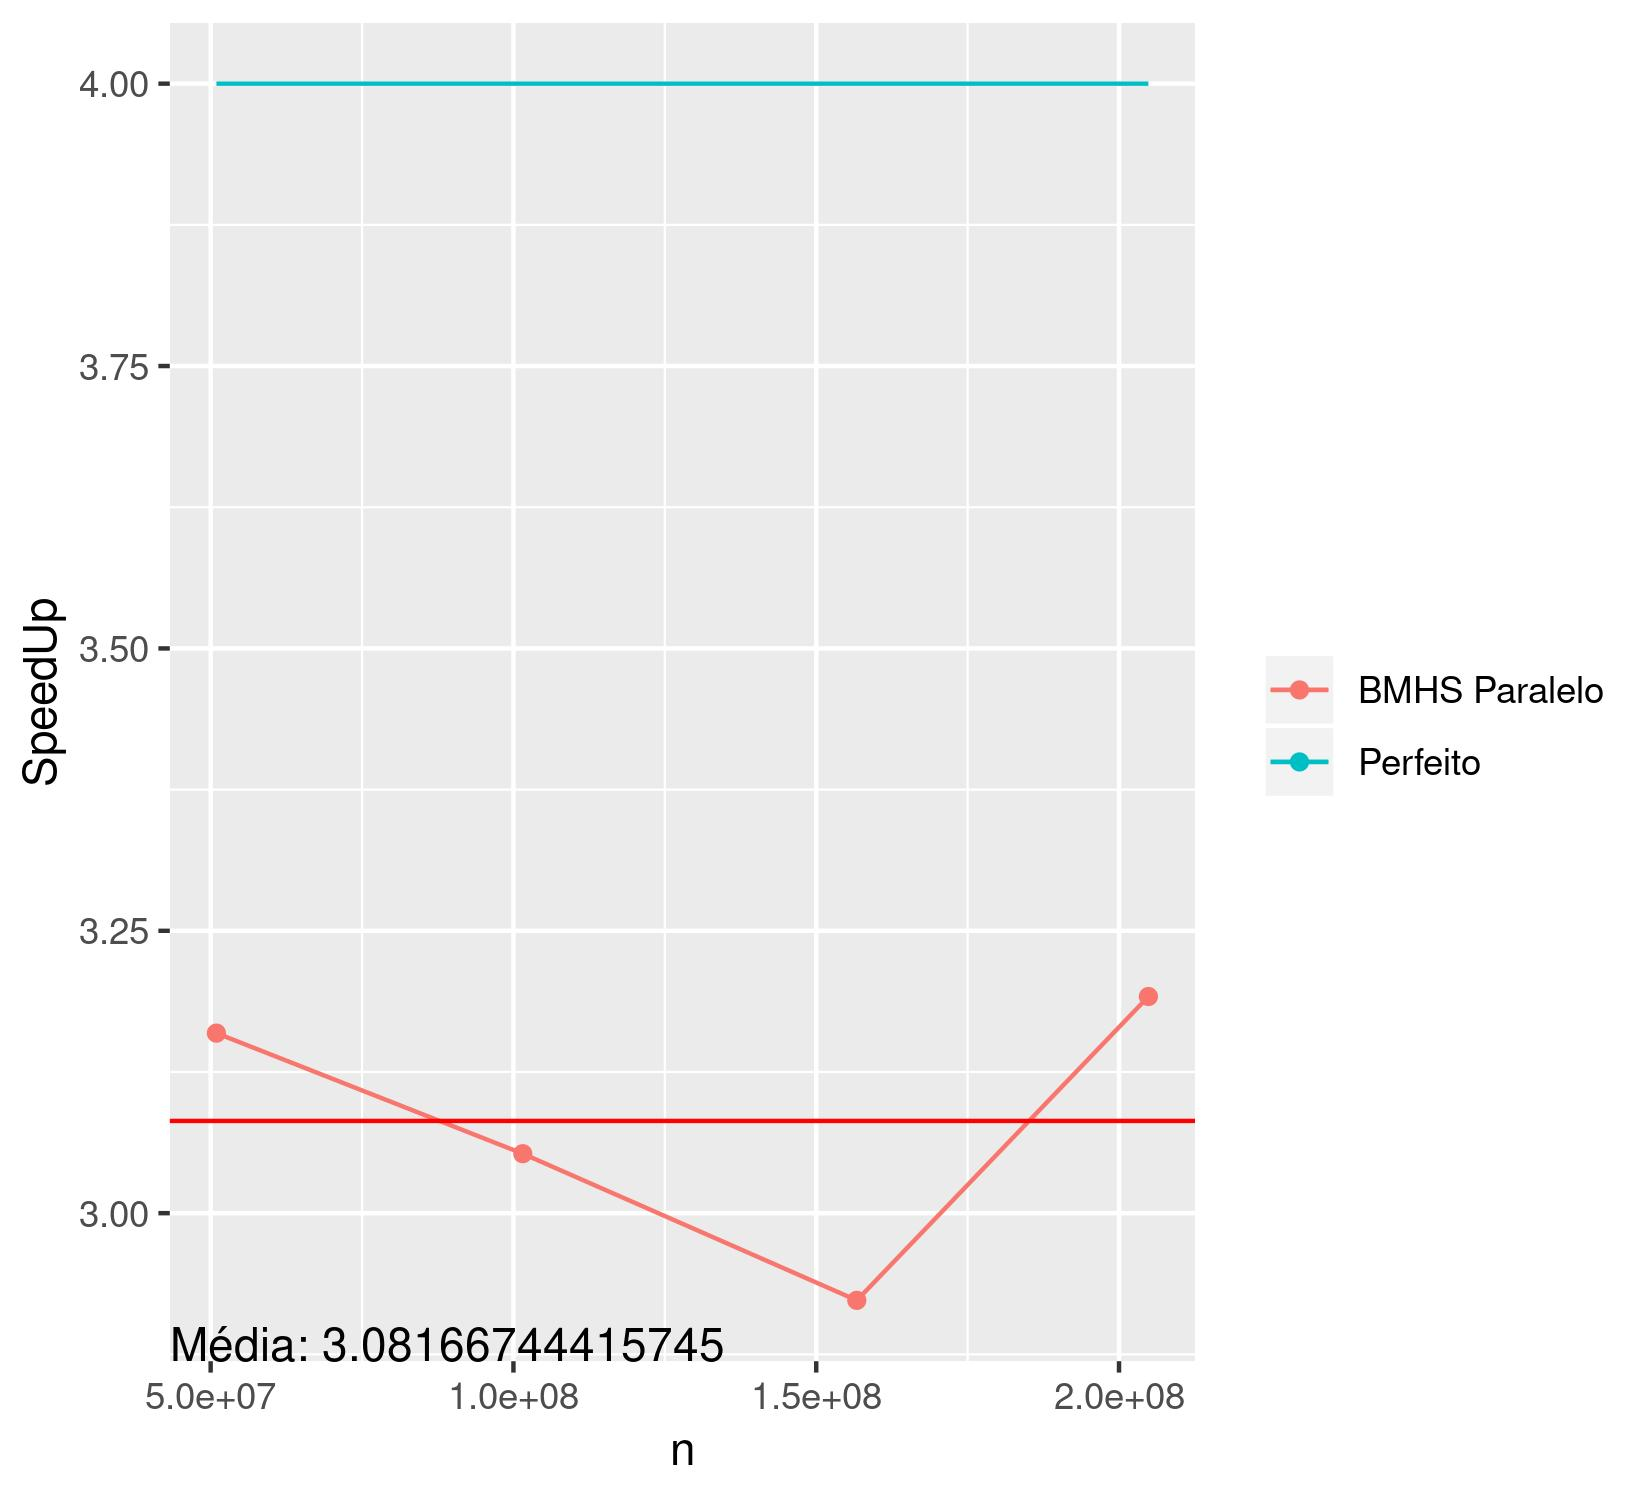
\includegraphics[width=5.5cm]{nxspeedup}
\caption{m=30,p=4.}\label{fig:nxspeedup}
\end{subfigure}
\begin{subfigure}[b]{.33\linewidth}
\centering
\caption{p=2,base $\iota$.}\label{fig:mxspeedup2p}
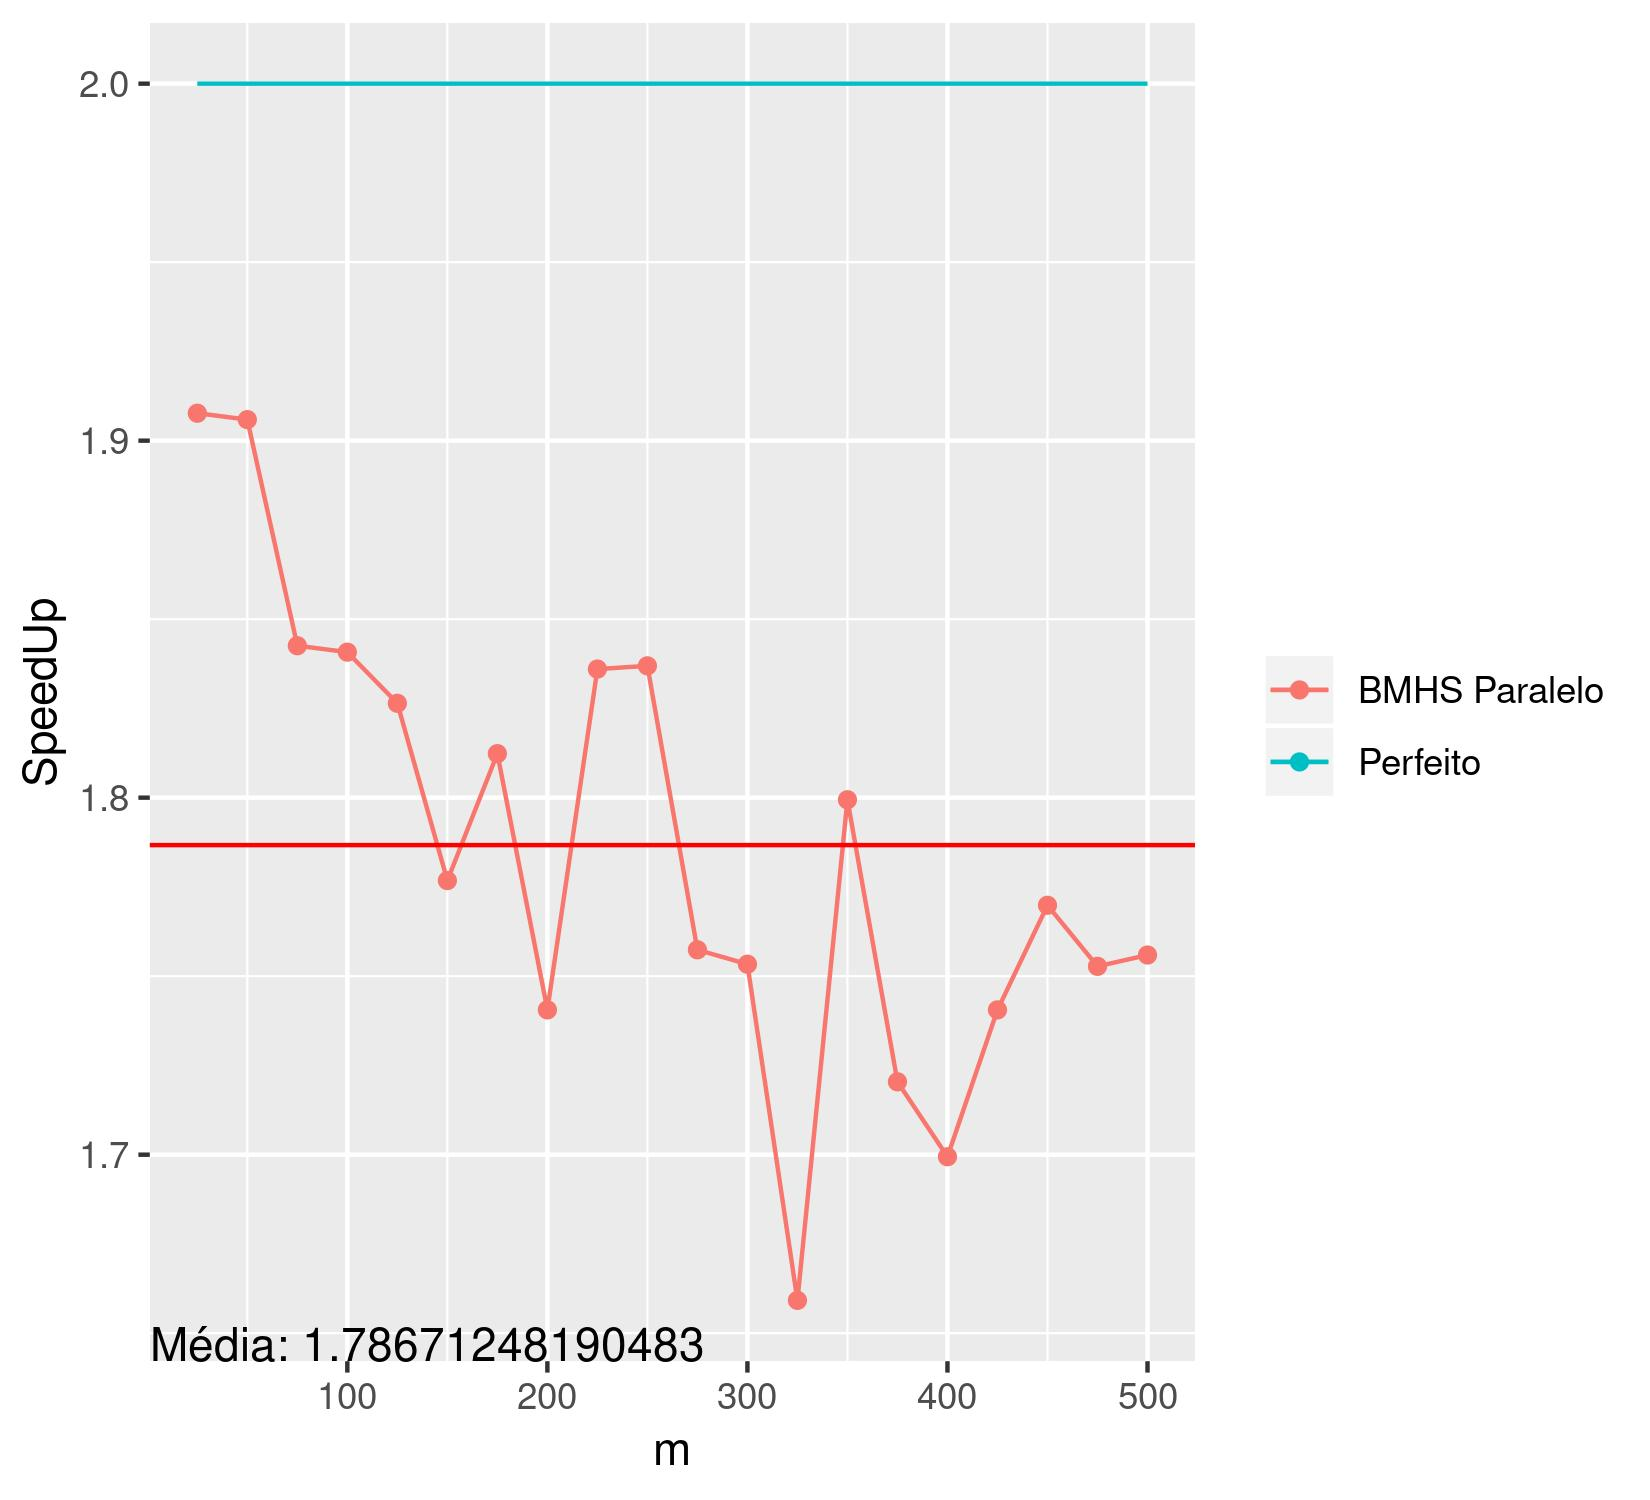
\includegraphics[width=5.5cm]{mxspeedup2p}
\end{subfigure}
\caption{Speedup.}
\end{figure}
\end{center}

\subsection{Espaço}
\label{sec:org2ea6658}

Para provar a complexidade de espaço do algoritmo principal basta monitorar as alocações feitas pelo algoritmo para cada tamanho de entrada. O monitoramento será feito somente da memória \emph{heap} \cite{osthreeeasypieces} que é a parte da memória onde a alocação dinâmica é feita e o espaço pode-se variar dinamicamente permitindo-se assim obter uma função de complexidade correta.

Na figura \ref{fig:mxbytes} é comprovado que \(m\) influência na complexidade de espaço dos algoritmos. Também é possível ver o salto que há no uso de memoria do ShiftAnd de acordo com que é necessário alocar blocos de \(\beta\) bits. É possivel observar que o BMH, BMHS e BMHS Paralelo compartilham da mesma função de uso de bytes, isso se deve a eles usarem somente o espaço de alocar o padrão no programa principal.

A figura \ref{fig:nxbytes} mostra também que todos algoritmos somente alocam o texto no programa principal, por isso todos possuem a mesma função em relação a variável n.

As figuras \ref{fig:errorxbytes} e \ref{fig:pxbytes} comprovam o fator de erro e de número de processadores na complexidade de espaço dos algoritmos ShiftAnd e BMHS paralelo respectivamente.

\begin{center}
\begin{figure}
\begin{subfigure}[b]{.49\linewidth}
\centering
\caption{base=$\zeta$.}\label{fig:mxbytes}
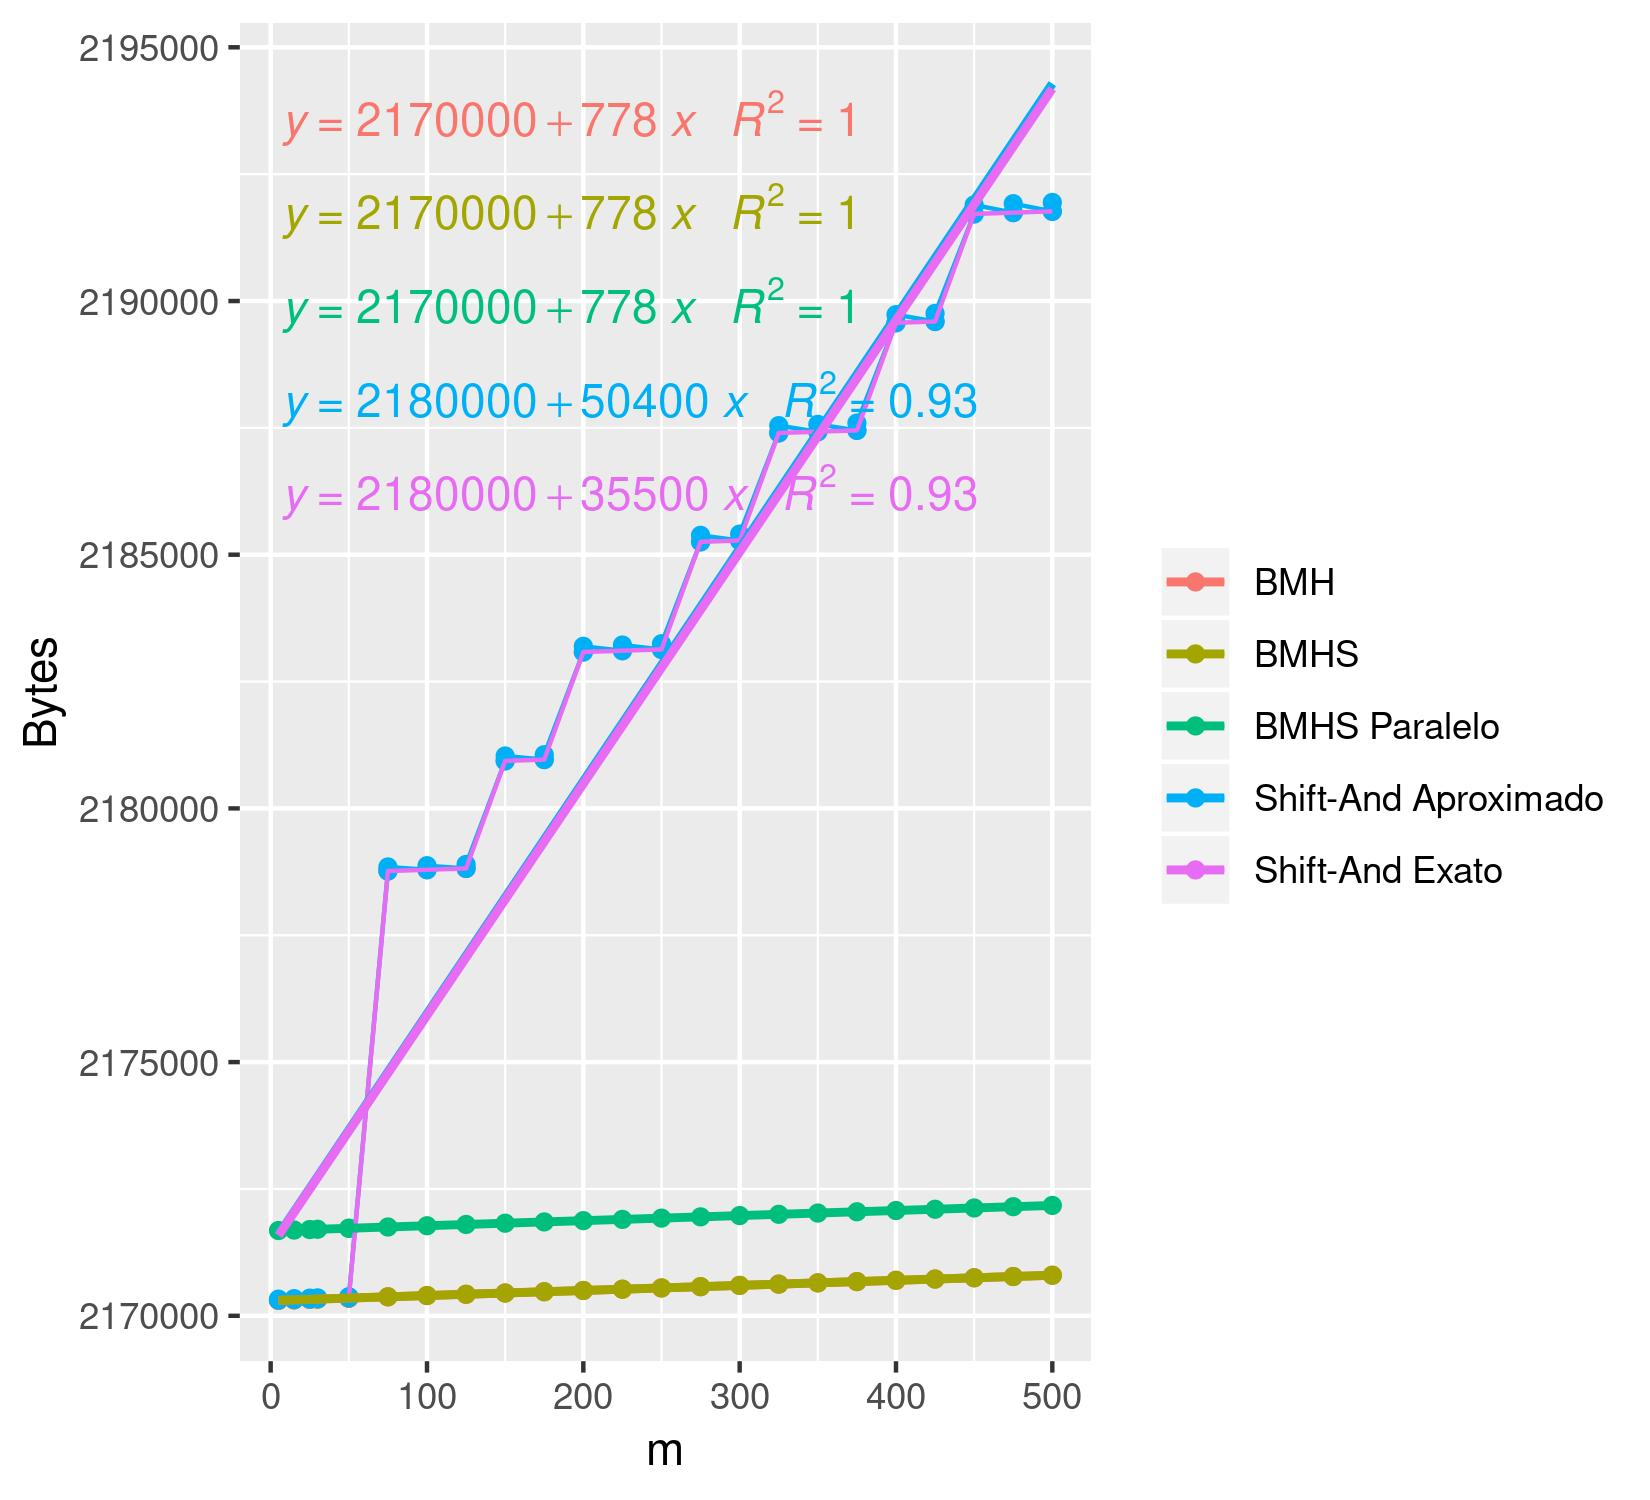
\includegraphics[width=4.4cm]{mxbytes}
\end{subfigure}
\begin{subfigure}[b]{.49\linewidth}
\centering
\caption{m=30.}\label{fig:nxbytes}
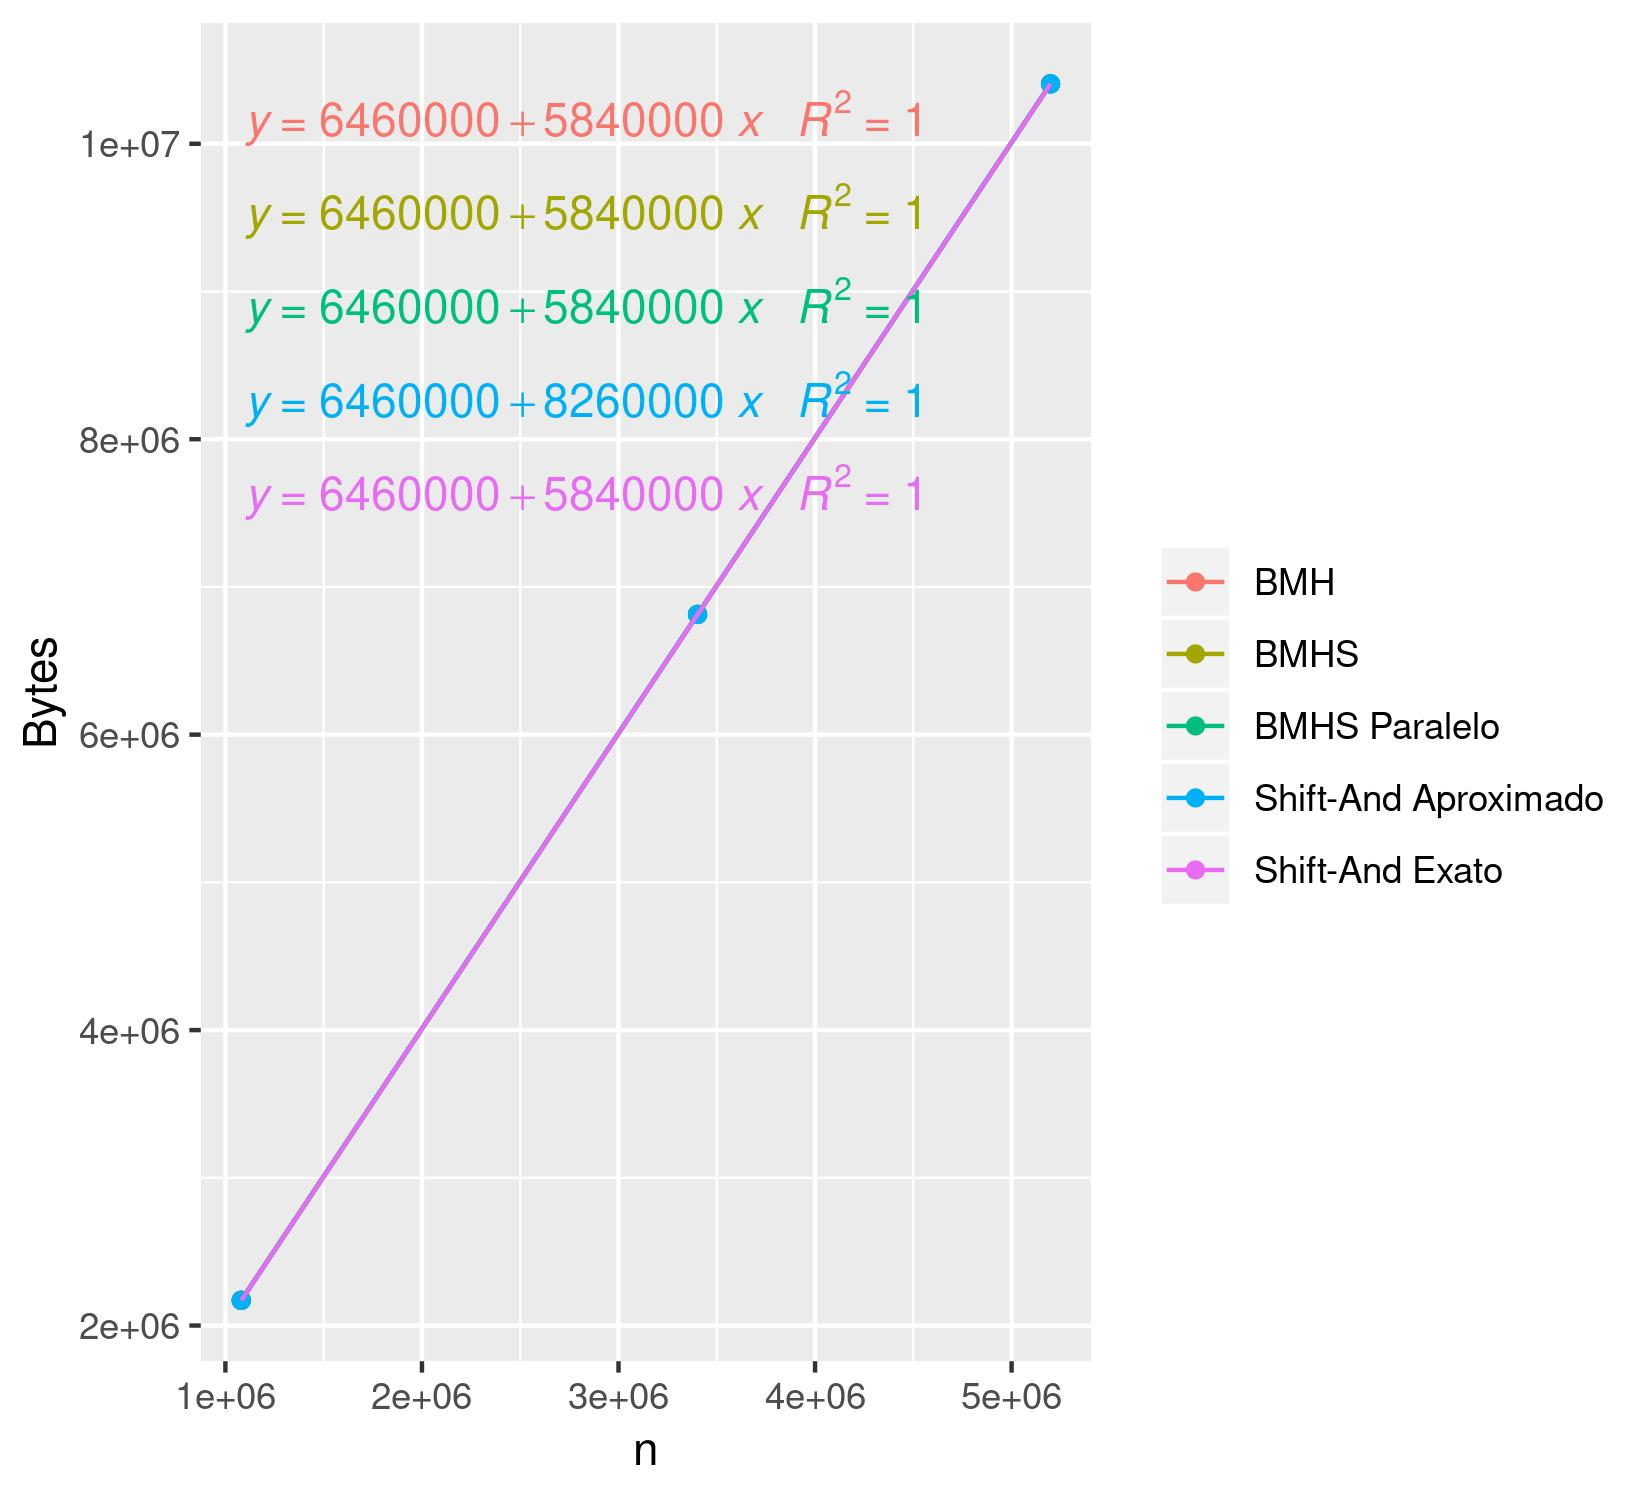
\includegraphics[width=4.4cm]{nxbytes}
\end{subfigure}
\begin{subfigure}[b]{.49\linewidth}
\centering
\caption{base=$\zeta$,m=30.}\label{fig:errorxbytes}
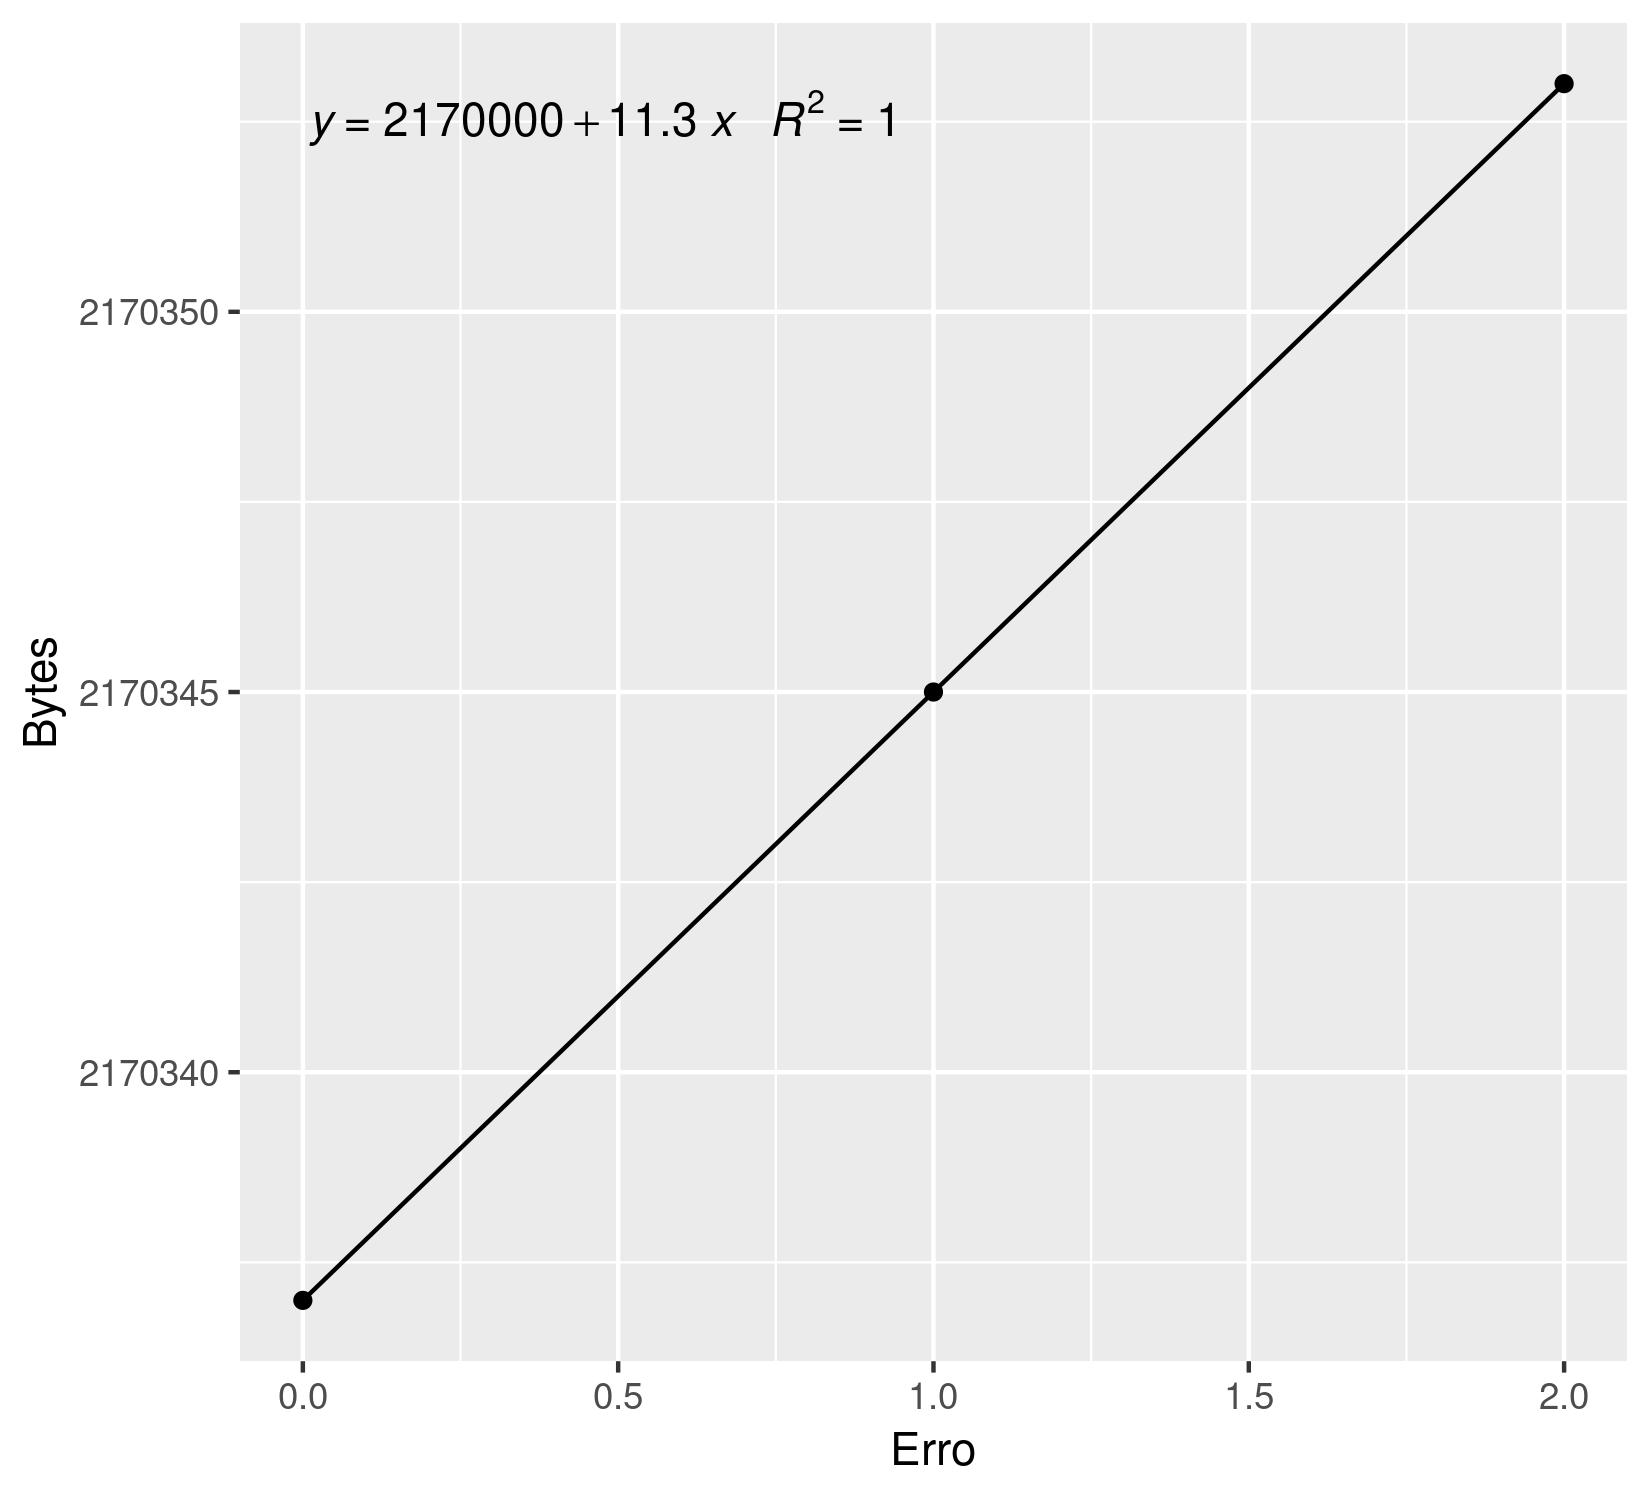
\includegraphics[width=3.5cm]{errorxbytes}
\end{subfigure}
\begin{subfigure}[b]{.49\linewidth}
\centering
\caption{base=$\zeta$,m=30.}\label{fig:pxbytes}
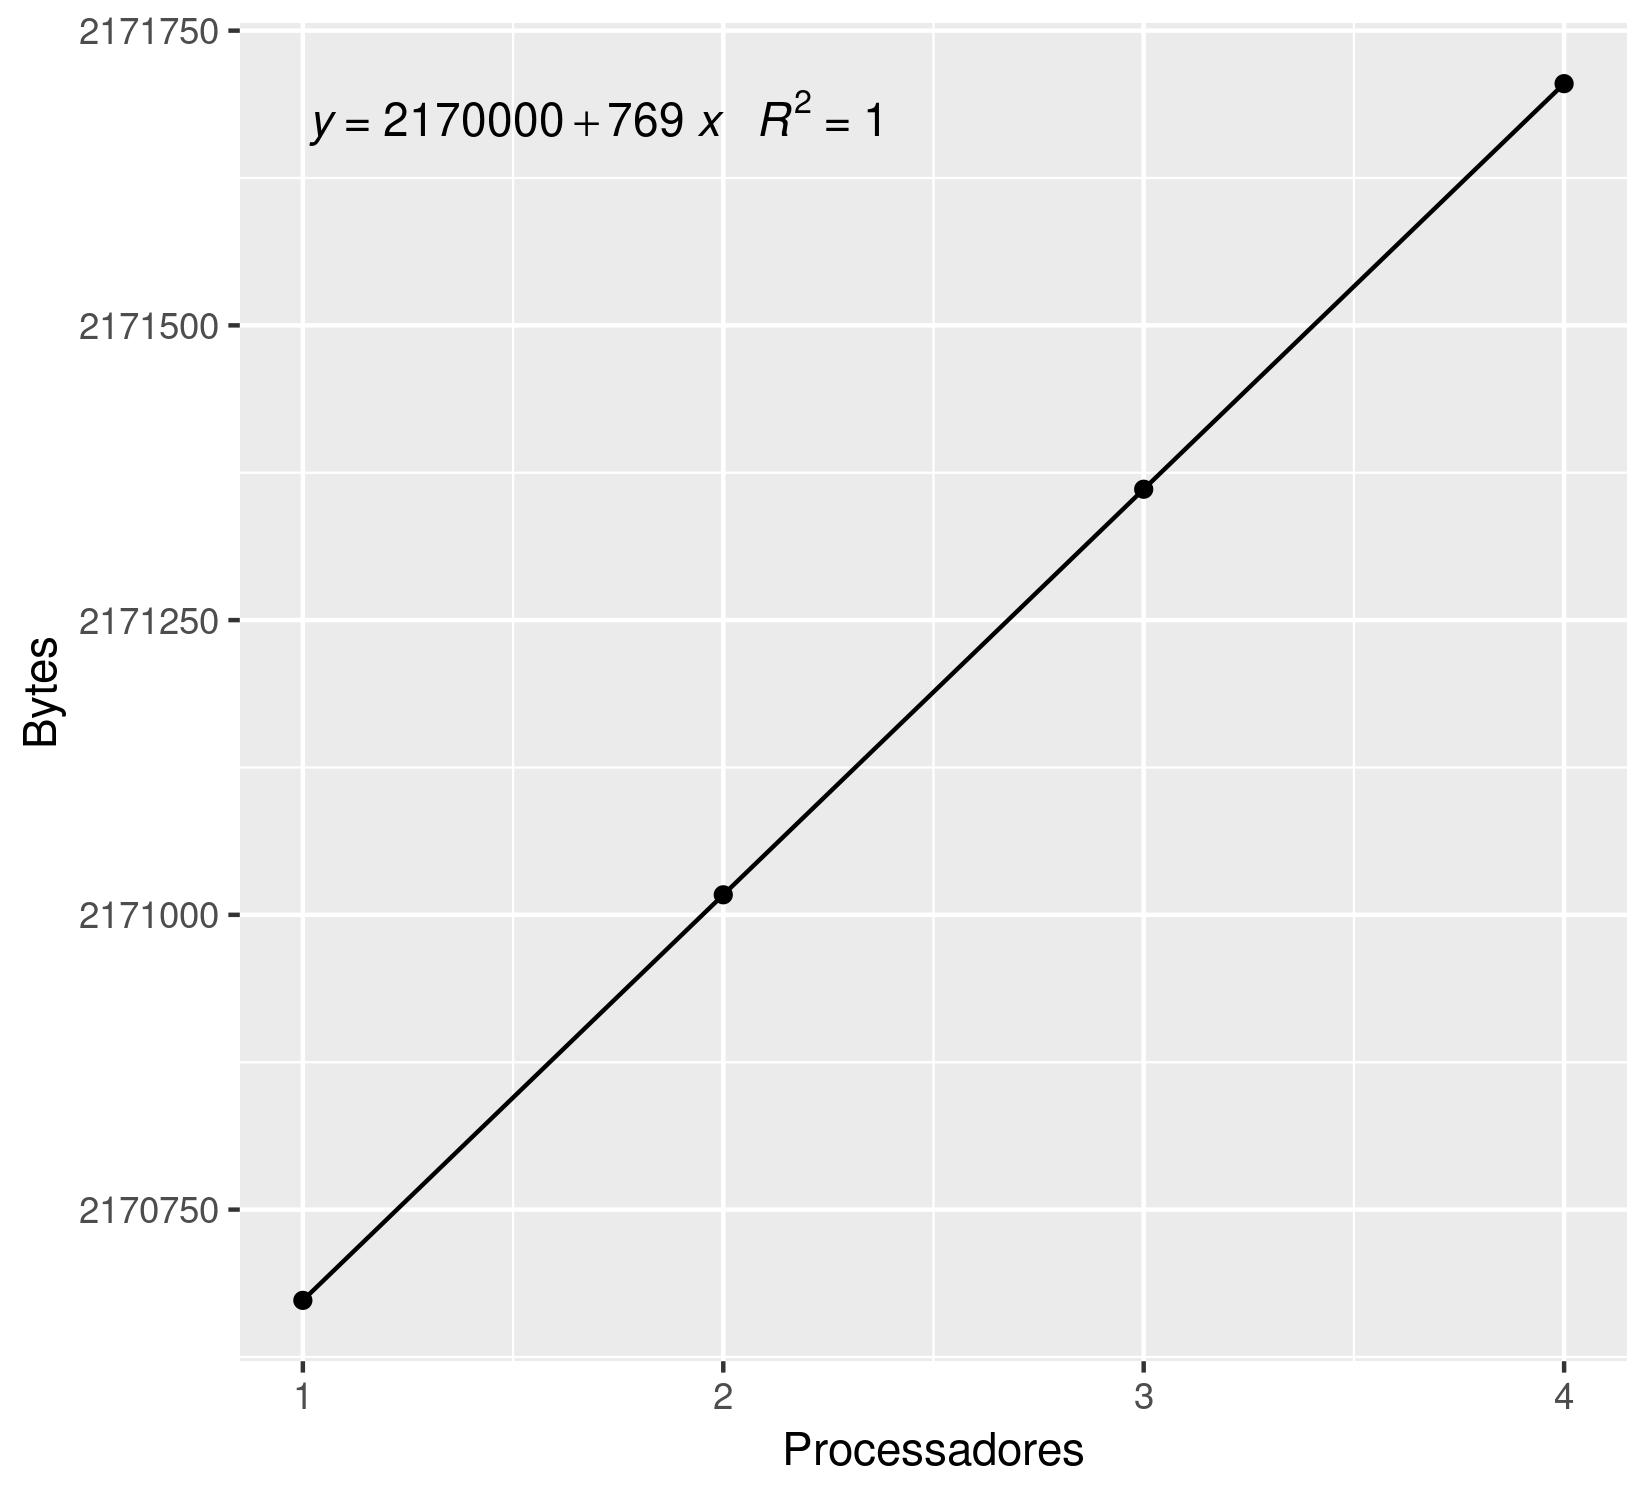
\includegraphics[width=3.5cm]{pxbytes}
\end{subfigure}
\caption{Espaço utilizado pelos algoritmos em termos de diversos fatores.}
\end{figure}
\end{center}


\subsection{Análise geral}
\label{sec:orgc039873}

Com os algoritmos analisados e mostrados suas eficiências na prática pode-se criar uma hierarquia dos mesmos para cada situação. Veja a figura \ref{fig:hierarquia}.

Para casos médios o BMHS Paralelo foi o mais rápido dentre todos, porém se for o pior caso esse algoritmo não é tão bom assim porém não é o pior de todos algoritmos.

Em casos médios o BMH é um bom algoritmo, porém não há muitas diferenças dele para o BMHS, em relação a desempenho, somente em casos específicos um supera o outro.

Já o ShiftAnd quando no pior caso ele é consideravelmente mais rápido que os outros algoritmos pois sua complexidade não depende do padrão, porém em casos médios esse algoritmo é extremamente lento comparado aos outros, ainda mais se for Shift-And aproximado.

\begin{center}
\begin{figure}
\begin{subfigure}[b]{.49\linewidth}
\centering
\caption{Caso médio empírico.}
\begin{tikzpicture}
\node[draw,rectangle,minimum width = 3.5cm] (n1) {BMHS Paralelo};
\node[draw,rectangle,minimum width = 3.5cm,yshift=-0.5cm] (n2) {BMHS};
\node[draw,rectangle,minimum width = 3.5cm,yshift=-1cm] (n3) {BMH};
\node[draw,rectangle,minimum width = 3.5cm,yshift=-1.55cm] (n4) {Shift-And};
\draw[<-,line width=0.3mm,right of = n1,xshift=1cm,yshift=0.27cm] (0,0) -- (0,-2.1) node[anchor=south west] {Rapidez};
\end{tikzpicture}
\end{subfigure}
\begin{subfigure}[b]{.49\linewidth}
\centering
\caption{Pior caso empírico.}
\begin{tikzpicture}
\node[draw,rectangle,minimum width = 3.5cm] (n1) {Shift-And};
\node[draw,rectangle,minimum width = 3.5cm,yshift=-0.5cm] (n2) {BMHS Paralelo};
\node[draw,rectangle,minimum width = 3.5cm,yshift=-1cm] (n3) {BMHS};
\node[draw,rectangle,minimum width = 3.5cm,yshift=-1.55cm] (n4) {BMH};
\draw[<-,line width=0.3mm,right of = n1,xshift=1cm,yshift=0.27cm] (0,0) -- (0,-2.1) node[anchor=south west] {Rapidez};
\end{tikzpicture}
\end{subfigure}
\caption{Hierarquia de tempo empírico.}\label{fig:hierarquia}
\end{figure}
\end{center}

\section{Conclusão}
\label{sec:org39b1144}

Com esse trabalho foi possível estudar a complexidade e o funcionamento dos algoritmos BMH,BMHS,Shift-And,Shift-And aproximado, BMHS paralelizado. Foi possível ver que o BMH e BMHS com complexidades piores que o Shift-And ainda sim conseguem na prática ser melhor que o Shift-And. A complexidade esperada de \(O(n/m)\) do algoritmo BMH e BMHS também foram vistas na prática e suas superioridades em relação ao Shift-And.

Os algoritmos foram classificados baseados nos desempenhos dos resultados, sendo o BMHS Paralelo o melhor algoritmo para casos médios e o Shift-And o melhor algoritmo para o pior caso.

Uma distribuição de blocos de memória foi modelada para o algoritmo BMHS Paralelo essa distribuição de blocos foi analisada de diversas formas, criando diversas funções que descrevem suas características, exemplo: seu tamanho total de blocos, taxa de blocos redundantes e etc. O BMHS paralelo obteve um speedup bom, sendo ele \(S_{4}\approx 3.18\) com 4 processadores e \(S_{2}\approx 1.78\) com 2 processadores.

Os algoritmos foram aplicados em genomas e esse estudo pode ser utilizado em outros trabalhos que aplique os algoritmos a outras áreas e as comparem.

Em futuros trabalhos pode-se estudar os efeitos da busca em arquivos comprimidos e todos seus impactos profundamente através dessa base que foi estudada nesse trabalho.

\bibliographystyle{plain}
\bibliography{doc}
\end{document}
